% Copyright (C) 2010-2013, Maximiliano Curia <maxy@gnuservers.com.ar>,
%               2010-2013, Margarita Manterola <marga@marga.com.ar>

% Esta obra está licenciada de forma dual, bajo las licencias Creative
% Commons:
%  * Atribución-Compartir Obras Derivadas Igual 2.5 Argentina
%    http://creativecommons.org/licenses/by-sa/2.5/ar/
%  * Atribución-Compartir Obras Derivadas Igual 3.0 Unported
%    http://creativecommons.org/licenses/by-sa/3.0/deed.es_AR.
%
% A su criterio, puede utilizar una u otra licencia, o las dos.
% Para ver una copia de las licencias, puede visitar los sitios
% mencionados, o enviar una carta a Creative Commons,
% 171 Second Street, Suite 300, San Francisco, California, 94105, USA.

\documentclass[11pt,spanish,a4paper]{report}
\tolerance=5000
%\renewcommand{\baselinestretch}{1.3}

% Entrada de texto
\usepackage[utf8]{inputenc}   % Permite escribir directamente áéíóúñ
\usepackage[spanish]{babel}   % Traduce los textos a castellano
\usepackage{t1enc}            % Agrega caracteres extendidos al font

% Cuestiones de estilo
\usepackage{palatino}         % Cambia el font por omision a Palatino
\usepackage{graphicx}         % Permite insertar imagenes.
\usepackage{listingsutf8}     % Permite mostrar codigo de forma mas linda
\usepackage{verbatim}         % Permite incluir archivos de texto verbatim

% Opcionales
\usepackage{longtable}         % tablas largas y flexibles
\usepackage{nonfloat}          % Hace que las figuras no floten
%\usepackage{fancyvrb}         % Agrega más entornos verbatim
%\usepackage{stmaryrd}         % Agrega más símbolos matemáticos
%\usepackage{enumerate}        % Agrega flexibilidad a las enumeraciones
%\usepackage{ifthen}           % Permite usar condicionales en comandos
%\usepackage{subfigure}        % Permite subfiguras dentro de las figuras

% Paquetes matematicos.  Hacen falta?
\usepackage{amsmath, amsthm, amssymb} % Se usan para theoremstyle

% Margenes y largo del texto
%
% medidas horizontales
% 1in(fijo) + \hoffset + \(odd|even)sidemargin + \textwidth + \marginparsep +
% \marginparwidth + \marginparpush
%
% medidas verticales
% 1in(fijo) + \voffset + \topmargin + \headheight + \headsep + \textheight +
% \footskip

\setlength\oddsidemargin{-0.04cm}
\setlength\evensidemargin{-0.04cm}
\setlength\topmargin{0cm}
\setlength\headheight{0.5cm}
\setlength\headsep{0.3cm}
\setlength\footskip{0.8cm}
\setlength\textwidth{16cm}  % ancho para apunte
\setlength\textheight{23cm} % largo para apunte
%\leftmargin 2.5cm
%\rightmargin 2.5cm

\usepackage{fancyhdr}         %
\pagestyle{fancy}
\fancyhf{} % clear all header and footer fields
\fancyhead[RO]{\slshape \rightmark \hspace{1cm} \normalfont \bfseries \thepage}
\fancyhead[LE]{\bfseries \thepage \hspace{1cm} \normalfont \leftmark}
%\fancyfoot{} % clear all footer fields
%\fancyfoot[RO]{\bfseries \thepage}
%\fancyfoot[LE]{\bfseries \thepage}
\renewcommand{\headrulewidth}{0.3pt}
\renewcommand{\footrulewidth}{0pt}

\fancypagestyle{plain}{%
\fancyhf{} % clear all header and footer fields
\fancyfoot[RO]{\bfseries \thepage}
\fancyfoot[LE]{\bfseries \thepage}
\renewcommand{\headrulewidth}{0pt}
\renewcommand{\footrulewidth}{0pt}}

% Encabezado en la parte superior de las hojas
\renewcommand{\sectionmark}[1]{\markright{\thesection.\ #1}}
\renewcommand{\chaptermark}[1]{\markboth{\chaptername\ \thechapter.\ #1}{}}

% Cuadros de observación
\newcommand{\Observacion}[1]{
\begin{center}
\begin{tabular}[c]{|c|}\hline
#1\\ \hline
\end{tabular}
\end{center}
}

\usepackage{color}            % Permite definir colores
\definecolor{celeste}{rgb}{0.90,0.90,0.95}
\definecolor{verde}{rgb}{0.85,1.00,0.85}
\definecolor{amarillo}{rgb}{1.00,1.00,0.85}

% Caja temporal para guardar el texto - Que se usa en las cajas de texto
\newsavebox{\temporalbox}

% Cuadros de Sabias qué - Icono: lamparita
\newenvironment{sabias_que}
 {\begin{lrbox}{\temporalbox}\begin{minipage}{0.95\textwidth}
  \begin{minipage}{0.05\textwidth}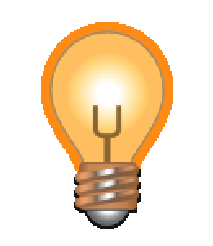
\includegraphics[height=4ex]{graficos/lamparita}\end{minipage}
  \begin{minipage}{0.80\textwidth}\bf Sabías que \ldots\end{minipage}\\
  \begin{small}}
 {\end{small}\end{minipage}\end{lrbox}
  \begin{figure*}[ht]
  \centering
  \fboxsep 0.5em
  \fcolorbox{black}{celeste}{
  \usebox{\temporalbox}}
  \end{figure*}}

% Cuadros de Atención - Icono: Triángulo con !
\newenvironment{atencion}
 {\begin{lrbox}{\temporalbox}\begin{minipage}{0.95\textwidth}
  \begin{minipage}{0.05\textwidth}
\includegraphics[height=3ex]{graficos/atencion}\end{minipage}
  \begin{minipage}{0.80\textwidth}\bf Atención \end{minipage}\vspace{0.8ex}\\
  \begin{small}}
 {\end{small}\end{minipage}\end{lrbox}
  \begin{figure*}[ht]
  \centering
  \fboxsep 0.5em
  \fcolorbox{black}{amarillo}{
  \usebox{\temporalbox}}
  \end{figure*}}

\usepackage{framed}           % Cuadros multihoja con color de fondo

% Cuadros de referencia del lenguaje. - Icono: logo python
\newenvironment{referencia_python}
 {\definecolor{shadecolor}{rgb}{0.85,1.00,0.85}%
  \begin{shaded}%
  \begin{minipage}{0.80\textwidth}\hspace{-1em}\bf Referencia del lenguaje Python\end{minipage}%
  \hfill%
  \begin{minipage}{0.05\textwidth}
\includegraphics[height=4ex]{graficos/logo-python}\end{minipage}\\
  \rule[1.00ex]{1.0\textwidth}{0.01ex}\\
  \vspace{-2ex}%
  \begin{small}}
 {\end{small}\end{shaded}}

\newenvironment{sintaxis}[1]
  {\hspace{-1em}\textbf{#1}%
   \vspace{1ex}\\
   \begin{minipage}{0.05\textwidth}\end{minipage}\hfill\begin{minipage}{0.90\textwidth}}
  {\end{minipage}\hfill\begin{minipage}{0.05\textwidth}\end{minipage}\\}

% Parametros para los listings de python
\lstset{language=C,
    numbers=left,
    numberstyle=\tiny,
    numbersep=5pt,
    showstringspaces=false,
    basicstyle=\ttfamily,
    inputencoding=utf8,
    literate=%
        {á}{{\'a}}1
        {é}{{\'e}}1
        {í}{{\'i}}1
        {ó}{{\'o}}1
        {ú}{{\'u}}1
        {ü}{{\"u}}1
        {Á}{{\'A}}1
        {É}{{\'E}}1
        {Í}{{\'I}}1
        {Ó}{{\'O}}1
        {Ú}{{\'U}}1
        {Ü}{{\"U}}1
        {ñ}{{\~n}}1
        {Ñ}{{\~N}}1
        {¡}{{!`}}1
        {¿}{{?`}}1
}
%    basicstyle=\ttfamily\normalsize,
%    keywordstyle=\ttfamily\bfseries,
%    identifierstyle=\ttfamily,
%    commentstyle=\ttfamily\itshape,
%    stringstyle=\ttfamily,

\usepackage{float}            % Agrega estilos a los floats

\floatstyle{ruled}
\newfloat{codigo-float}{thp}{lop}
\floatname{codigo-float}{Código}

\newenvironment{codigo}[2]{\begin{codigo-float}
    \caption{{\small\texttt{#1}}\textbf{:}\ \small #2}
    }{\end{codigo-float}}

\lstnewenvironment{codigo-c}{\lstset{xleftmargin=10pt,tabsize=4}}{}
\lstnewenvironment{codigo-c-plano}{\lstset{xleftmargin=10pt,tabsize=4,numbers=none}}{}

% Numeracion para secciones y subsecciones - Hace falta?
%\renewcommand{\thesection}{\thechapter.\arabic{section}}
%\renewcommand{\thesubsection}{\thesection.\arabic{subsection}}

% Estilos usados en el texto
\theoremstyle{definition}
\newtheorem{definicion}{Definici\'on}[section]
\newtheorem{ejemplo}{Ejemplo}[section]
\newtheorem{problema}{Problema}[section]
\newtheorem{ejercicio}{Ejercicio}[section]
\newtheorem{ejerciciof}{}[section]
\newtheorem{problemac}{Problema}[chapter]
\newtheorem{ejercicioc}{Ejercicio}[chapter]
\renewcommand{\qedsymbol}{} % El proof inserta dos qed al final
\newenvironment{solucion}[1][Solución]{\begin{proof}[#1]}{\end{proof}}

\theoremstyle{remark}
\newtheorem{observacion}{Observaci\'on}[section]
\newtheorem{nota}{Nota}[section]

% Traducciones propias
\addto\captionsspanish{
\renewcommand{\chaptername}{Unidad}
\renewcommand{\contentsname }{Contenidos }
}

% Definiciones varias - En uso
\def\esp{\hspace{0.5ex}}
\def\ra{\rightarrow}
\def\qq{\textquoteright}

\begin{document}

% Carat no esta.
%\include{carat}
%\title{Algoritmos y Programación II \\ Con lenguaje C}
%\maketitle

%\tableofcontents  %Comentar  para no imprimir la toc

% Comando para configurar el número de capítulo
%\setcounter{chapter}{11}

% Copyright (C) 2010-2013, Maximiliano Curia <maxy@gnuservers.com.ar>,
%               2010-2013, Margarita Manterola <marga@marga.com.ar>

% Esta obra está licenciada de forma dual, bajo las licencias Creative
% Commons:
%  * Atribución-Compartir Obras Derivadas Igual 2.5 Argentina
%    http://creativecommons.org/licenses/by-sa/2.5/ar/
%  * Atribución-Compartir Obras Derivadas Igual 3.0 Unported
%    http://creativecommons.org/licenses/by-sa/3.0/deed.es_AR.
%
% A su criterio, puede utilizar una u otra licencia, o las dos.
% Para ver una copia de las licencias, puede visitar los sitios
% mencionados, o enviar una carta a Creative Commons,
% 171 Second Street, Suite 300, San Francisco, California, 94105, USA.

\renewcommand{\chaptermark}[1]{\markboth{#1}{}}
\renewcommand{\thesection}{\arabic{section}}
\chapter*{El lenguaje C}

En este apunte se dará una introducción básica al lenguaje de programación C,
asumiendo un conocimiento previo de técnicas de programación en algún otro
lenguaje.

\section{Características básicas del lenguaje}

Se podría decir que el lenguaje de programación C es un lenguaje
\textit{sencillo}, fácil de cubrir en poco tiempo, ya que tiene pocas palabras
reservadas, y una biblioteca estándar más acotada que la de otros lenguajes.

Sin embargo, la especificación actual contiene 701 páginas
\footnote{http://www.open-std.org/jtc1/sc22/wg14/www/docs/n1570.pdf} y es
posible crear código extremadamento \textit{ofuscado}
\footnote{http://www.ioccc.org/}, de modo que no es realmente correcto decir
que es sencillo. \\

C es un lenguaje de programación estructurado, de medio nivel, y muy portable.
Esto se debe a que el modelo de computadora que usa el lenguaje se puede
ajustar a una gran variedad de equipos. A veces se lo considera como un
lenguaje ensamblador de alto nivel, ya que el programador suele tener que
tener en cuenta detalles sobre cómo se representan los elementos del programa en
la máquina, o manejar (pedir y liberar) los recursos del sistema desde el
código.

\section{Estándares del lenguaje}

A lo largo de la historia se han desarrollado tres estándares principales.
\footnote{El último estándar del lenguaje es C11, publicado en el 2011, sin
embargo todavía no tuvo un impacto notable, por lo que nos concentraremos en
C99.}

\begin{description}
\item[K\&R] El estándar publicado en la primera edición del libro
''El lenguaje de programación C'' de Kernighan y Ritchie.
\item[C89] Publicado en la referencia estándar ANSI X3.159-1989 y luego en el
estándar ISO/IEC 9899:1990, así como en la segunda edición del mismo libro.
\item[C99] El estándar ISO, publicado en 1999.
\end{description}

Si bien a esta altura la mayoría de los compiladores de C soportan
prácticamente el estándar completo de C99
\footnote{http://gcc.gnu.org/c99status.html}, una gran parte de código
disponible utiliza todavía el estándar C89; es por eso que en este apunte se
hace especial distinción con aquellos detalles que pertencen al estándar C99.

\section{Tipos básicos}

C cuenta con una variedad de tipos numéricos.  De estos, los tipos enteros
pueden tomar los modificadores \lstinline!signed! o \lstinline!unsigned! para
indicar si son o no signados.

A continuación una tabla con los distintos tipos de C, ordenados según el
espacio que ocupan en memoria.

\begin{description}
\item[bool]
 Se agregó en C99. Puede contener los valores 0 y 1. Incluyendo la biblioteca
\lstinline!<stdbool.h>!, se pueden utilizar los valores \lstinline!true! y
\lstinline!false! (equivalentes a 1 y 0 respectivamente).

\item[char]
 Tipo entero, por omisión \lstinline!unsigned!, de tamaño de 1 byte.

\item[short]
 Tipo entero, por omisión \lstinline!signed!, debe ocupar menos espacio o el
mismo que int. En el compilador gcc, arquitectura Intel 32 bits, mide 16 bits.

\item[int]
 Tipo entero, por omisión \lstinline!signed!, es el tipo \textit{natural} de la
 arquitectura. En el compilador gcc, arquitectura Intel 32 bits, mide 32 bits.

\item[long]
 Tipo entero, por omisión \lstinline!signed!, debe ocupar igual o más espacio
que long. En el compilador gcc, arquitectura Intel 32 bits, mide 32 bits.

\item[long long]
 Tipo entero, por omisión signed, debe ocupar igual o más espacio
 que long. En el compilador gcc, arquitectura Intel 32 bits, mide 64 bits.

\item[float]
 Tipo real, cumple con el estándar IEEE 754 de simple precisión (32 bits).

\item[double]
 Tipo real, cumple con el estándar IEEE 754 de doble precisión (64 bits).

\item[long double]
 Tipo real, según la arquitectura y las opciones de compilación, puede cumplir
con el estándar IEEE 754 de doble precisión (64 bits) o de doble precisión
extendida (más de 79 bits, 80 bits en arquitecturas Intel 32 bits).

\item[complex]
 Se agregó en C99, representa un número complejo.  Ocupa dos
\lstinline!doubles!, y requiere incluir \lstinline!<complex.h>!

\item[float complex]
 Se agregó en C99, de menor tamaño que el complejo
común. Ocupa dos floats, también requiere \lstinline!<complex.h>!.

\item[long complex]
 Se agregó en C99, ocupa dos \lstinline!long doubles!, y también requiere
\lstinline!<complex.h>!.

\item[void]
 No se puede usar como un tipo de una variable, se usa
 para señalar que una función no devuelve nada o no recibe nada.
\end{description}

Además, se puede utilizar el modificador de \lstinline!const! para declarar
una variable que puede inicializarse pero una vez inicializada no puede
modificarse.

La inicialización de las variables se realiza cuando se definen. En el caso
de las funciones, los valores que reciben los parámetros actuan como
inicializadores.

\section{Sintáxis básica}

Asumiendo conocimientos previos de programación, se describe a continuación la
sintaxis básica del lenguaje de programación C.

\subsection{Instrucciones}

Las instrucciónes en C son lo que forman las secuencias que ejecutarán los
programas, las instrucciones terminan en \lstinline!;! y donde puede haber una
instrucción puede haber también una serie de instrucciones entre llaves:
\lstinline!{! (para comenzar el bloque) y \lstinline!}! (para terminar el
bloque).

\subsection{Valores literales}

Los valores literales son valores explícitamentes escritos en el código.
Y merecen un breve comentario en este resumen.

Los valores númericos se pueden escribir en decimal (\lstinline!4095!), en
octal (\lstinline!07777!) o en hexadecimal (\lstinline!0xFFF!). Además, se les
puede agregar al final una \lstinline!L! para indicar que es un
\lstinline!long! o una \lstinline!U! para indicar que es un valor
\lstinline!unsigned!.

En el caso de los valores reales, se los puede representar con punto como
separador entre parte entera y decimal o en notación científica. Por omisión,
estos valores serán de tipo \lstinline!double!, pero se puede usar una letra
\lstinline!F! como sufijo del valor para que se los tome como
\lstinline!float!.

Los caracteres también son valores numéricos, pero se pueden escribir a través
del símbolo que representan escribiéndolos entre comillas simples. Asumiendo
que se utiliza un sistema en ASCII, \lstinline!'A'! será lo mismo que escribir
el valor 65.  Varios de los caracteres especiales (como el fin de línea) se
pueden representar en C como una secuencia de \lstinline!\!  seguida de algún
caracter, por ejemplo, el fin de línea se representa como \lstinline!'\n'!.

A continuación una tabla con las secuecias que representan caracteres
especiales.

\begin{tabular}{ccl}
Secuencia & Nombre & Descripción \\
\hline
\lstinline!\n! &  NL & fin de línea (enter) \\
\lstinline!\t! &  HT & tabulación horizontal (tab) \\
\lstinline!\v! &  VT & tabulación vertical \\
\lstinline!\b! &  BS & retroceso (backspace) \\
\lstinline!\r! &  CR & retorno de carro \\
\lstinline!\f! &  FF & avance de hoja \\
\lstinline!\a! &  BEL & señal audible (beep) \\
\lstinline!\\! &  \verb!\! & contra barra \\
\lstinline!\'! &  \verb!'! & comillas simples \\
\lstinline!\0! &  NUL & caracter nulo \\
\lstinline!\ooo! & ooo & caracter con el valor octal ooo \\
\lstinline!\xHH! & HH  & caracter con el valor hexadecimal HH
\end{tabular}

Una cadena literal en C se escribe dentro de comillas dobles, por ejemplo
\lstinline!"ejemplo"! será un vector de 8 \lstinline!char!, el último de estos
caracteres será \lstinline!'\0'! (un caracter con valor entero 0).

\subsection{Estructuras Condicionales}

La estructura condicional evalúa la condición, si es verdadera ejecuta el
bloque verdadero, sino ejecuta el bloque alternativo.

En C, el condicional tiene dos formas básicas:

\begin{codigo-c-plano}
if (condición) {
    instrucciones;
}
\end{codigo-c-plano}

En este caso, el bloque se ejecuta únicamente si es verdadero y si no lo es,
no se ejecuta nada.  La otra opción es:

\begin{codigo-c-plano}
if ( condición ) {
    instrucciones-verdadero;
} else {
    instrucciones-falso;
}
\end{codigo-c-plano}

En ambos casos, cuando se trate de una única instrucción pueden omitirse las
llaves, pero en general se recomienda utilizarlas de todas maneras para
prevenir errores si luego se arreglan más instrucciones.

Una forma alternativa de la estructura condicional es la de múltiples
condiciones anidadas, que suele escribirse:

\begin{codigo-c-plano}
if ( condición_1 ) {
    cuerpo_1;
} else if ( condición_2 ) {
    cuerpo_2;
} else if ( condición_3 ) {
    cuerpo_3;
} else if ( condición_4 ) {
    cuerpo_4;
} else {
    cuerpo_else;
}
\end{codigo-c-plano}

Este tipo de estructura verifica las condiciones en cascada, hasta que una de
ellas sea verdadera y en ese caso se ejecutará el cuerpo correspondiente; de
no ser así, llegará al \lstinline!else! final.  Se trata únicamente de una
forma de escribir cómodamente los condicionales anidados.

Otra estructura de selección multiple es el \lstinline!switch!, que se muestra a
continuación.

\begin{codigo-c-plano}
switch ( expresión_entera ) {
case valor_entero_1:
    instrucciones;
    break;
case valor_entero_2:
    instrucciones;
    break;
...
default:
    instrucciones;
    break;
}
\end{codigo-c-plano}

En este caso, se compara la \lstinline!expresion_entera! con los distintos
valores enteros, y cuando coincide, se ejecutan las correspondientes
instrucciones.  De omitirse la instrucción \lstinline!break!, se continúa
ejecutando el siguiente bloque, sin importar que corresponda a otro valor.  En
el caso en que no coincida con ninguno de los valores, se ejecutará el bloque
\lstinline!default!.

Es importante notar que este tipo de selección multiple sólo puede operar con
enteros, de manera que tanto la expresión usada con la instrucción
\lstinline!switch! como cada uno de los posibles valores usados con
\lstinline!case! son tomados como enteros para compararlos.

\subsubsection{Concepto de verdadero}

El concepto de verdadero de C es \textit{todo lo que es 0 es falso, todo lo
demás en verdadero}.

En C99 existe el tipo \lstinline!bool! que es 0 en el caso de falso, y 1 en
caso de verdadero, pero no es necesario utilizar este tipo para las
condiciones, cualquier variable que valga 0 se considerará falsa, y cualquier
variable con un valor distinto de 0 se considerará verdadera.

\subsubsection{Operadores de comparación}

En C existen diversos operadores de comparación entre valores, a continuación
una tabla con los operadores más comunes.

\begin{tabular}{cl}
Operador & Significado \\
\hline
\lstinline!a1 == a2! & \lstinline!a1! vale lo mismo que \lstinline!a2! \\
\lstinline|a1 != a2| & \lstinline!a1! no vale lo mismo que \lstinline!a2! \\
\lstinline!a1 > a2! & \lstinline!a1! es mayor que \lstinline!a2! \\
\lstinline!a1 < a2! & \lstinline!a1! es menor que \lstinline!a2! \\
\lstinline!a1 >= a2! & \lstinline!a1! es mayor o igual que \lstinline!a2! \\
\lstinline!a1 <= a2! & \lstinline!a1! es menor o igual que \lstinline!a2! \\
\end{tabular}

Además, los operadores de comparación pueden unirse o modificarse para formar
expresiones más complejas.

\begin{tabular}{cl}
Operador & Significado \\
\hline
\lstinline!e1 && e2! & Debe cumplirse tanto \lstinline!e1! como \lstinline!e2! \\
\lstinline!e1 || e2! & Debe cumplirse \lstinline!e1!, \lstinline!e2! o ambas \\
\lstinline?! e1?     & \lstinline!e1! debe ser falso \\
\end{tabular}

Incluyendo la biblioteca \lstinline!<iso646.h>! se puede usar las palabras
\lstinline!and!, \lstinline!or!, \lstinline!not!, y otros, como operadores, de
la misma manera que son operadores en otros lenguajes.

\subsection{Ciclos}

El bucle \textit{mientras} en C tiene la siguiente forma:

\begin{codigo-c-plano}
while ( condición ) {
    cuerpo;
}
\end{codigo-c-plano}

La condición es evaluada en cada iteración, y mientras sea verdadera se
ejecuta el cuerpo del bucle.

También existe un bucle \lstinline!do...while!:

\begin{codigo-c-plano}
do {
    cuerpo;
} while ( condición );
\end{codigo-c-plano}

La diferencia con el anterior es que asegura que cuerpo va a ejecutarse al
menos una vez, ya que la condición se evalúa después de haber ejecutado el
cuerpo.

El lenguaje C cuenta con un bucle iterativo \textit{for}, un poco distinto a
otros bucles del mismo nombre.  Para comprenderlo mejor es importante notar
que las dos siguientes porciones de código son equivalentes:

\begin{codigo-c-plano}
for (inicialización; condición; incremento) {
    cuerpo;
}
\end{codigo-c-plano}

\begin{codigo-c-plano}
inicialización;
while (condición) {
    { cuerpo; }
    incremento;
}
\end{codigo-c-plano}

\subsection{Variables}

Todas las variables en C hay que declararlas antes de poder usarlas, la
declaración se hace de la siguiente manera:

\begin{codigo-c-plano}
tipo nombre_variable;
\end{codigo-c-plano}

Se pueden declarar varias variables del mismo tipo separandolas con comas.

\begin{codigo-c-plano}
tipo nombre_variable_1, nombre_variable_2;
\end{codigo-c-plano}

Además, es posible asignar un valor de inicialización al declararlas:

\begin{codigo-c-plano}
tipo nombre_variable_1 = valor_1 , nombre_variable_2 = valor 2;
\end{codigo-c-plano}

\subsection{Comentarios}

En C89 la única forma de poner comentarios es utilizando bloques que comiencen
con \lstinline!/*! y terminen con \lstinline!*/!. En C99, además, se agregó
soporte de comentarios \textit{hasta el final de la línea}, estos empiezan con
\lstinline!//!.

\subsection{Funciones}

Las funciones en C se definen de la siguiente manera:

\begin{codigo-c-plano}
tipo funcion (tipo_1 argumento_1, ..., tipo_n argumento_n)
{
    intrucciones;
    ...;
    return valor_retorno;
}
\end{codigo-c-plano}

Es decir que el tipo que devuelve la función se coloca antes del nombre de la
función, y luego se colocan los argumentos que recibe la función, precedidos
por su tipo.  En el caso de no recibir ningún argumento, se puede colocar
simplemente \lstinline!()! o \lstinline!(void)!.

El cuerpo de las funciones contendrá una secuencia de declaración de
variables, instrucciones, bloques, estructuras de control, etc.  \\

Una función debe estar declarada antes (leyendo el archivo desde arriba hacia
abajo) de poder llamarla en el código.  Es por esto que la definición (o
prototipo) de la función puede colocarse antes del contenido de la función, de
forma que pueda ser utilizada por funciones que se encuentran implementadas
antes.  En ese caso será:

\begin{codigo-c-plano}
tipo funcion (tipo_1 argumento_1, ..., tipo_n argumento_n);
\end{codigo-c-plano}

\subsection{Punto de entrada}

Se llama punto de entrada a la porción de código que se ejecuta en primer
lugar cuando se llama al programa desde la línea de comandos. En C el punto de
entrada es la función \lstinline!main! y dado que es una función que
interactúa con el sistema, tiene un prototipo en particular (con dos
opciones):

\begin{codigo-c-plano}
int main (void);
\end{codigo-c-plano}

Se puede ver que la función main devuelve un entero, que será el valor de
retorno del programa, 0 indicará que el programa se ejecutó exitosamente y
cualquier otro valor indicará un error. Esta opción, que no recibe parámetros,
se utiliza cuando no se quieren tener en cuenta los parámetros de línea de
comandos.  La otra opción se utiliza cuando sí se quieren tener en cuenta
estos parámetros:

\begin{codigo-c-plano}
int main (int argc, char *argv[]);
\end{codigo-c-plano}

En este caso, los parámetros \lstinline!argc! y \lstinline!argv! podrían tener
cualquier otro nombre, pero es convención usar estos dos. Su significado es
\emph{la cantidad de argumentos} y \emph{un vector de punteros a los
argumentos} respectivamente.  Más adelante se verán en detalle los temas de
vectores y punteros.


\section{Tipos derivados}

\subsection{Vectores}

Los vectores (o arreglos) son bloques continuos de memoria que contienen un
número de elementos del mismo tipo. Se los declara de la siguiente manera:

\begin{codigo-c-plano}
tipo_elemento nombre_vector[tamaño];
\end{codigo-c-plano}

Opcionalmente se puede inicializar el contenido:

\begin{codigo-c-plano}
tipo_elemento nombre_vector[] = { valor_0, valor_1, ... valor_n-1 };
\end{codigo-c-plano}

En este caso el tamaño es implícito, el compilador lo decide a partir de la
cantidad de elementos ingresada en el inicializador. \\

Para acceder al contenido de un vector se utiliza a través del índice del
elemento dentro del vector. Los índices del vector van desde 0 hasta
\lstinline!largo-1!.  Es importante recordar que \lstinline!vector[largo]! es
una posición inválida dentro del vector. Es decir:

\begin{codigo-c-plano}
tipo vector[largo];
vector[0] = valor; // asigna valor al primer elemento
valor = vector[9]; // toma el valor del décimo elemento
vector[largo-1] = valor; // asigna valor al último elemento
\end{codigo-c-plano}

Si se accede a un vector por su nombre, sin ningún índice, se obtiene
la posición en memoria del vector. Esto es una optimización para evitar tener
que hacer copias de (posiblemente) grandes bloques de memoria al llamar a una
función que recibe un vector. Esto tiene varias consecuencias:

\begin{itemize}
\item Los vectores se pasan como referencia, ya que lo que se pasa es la
posición de memoria donde se encuentra el vector.

\item Al recibir un vector en una función no hace falta definir el largo de
este, ya que el tamaño en memoria debería haber sido definido previamente.
\end{itemize}

Esto hace que en ciertas situaciones un vector tenga un comportamiento similar
al de los punteros, aunque no exactamente igual.

\subsection{Punteros}

Los punteros son direcciones de memoria. En C los punteros requieren tener un
tipo asociado, según el tipo de datos al que apuntan (es decir, el tipo de
datos que se encuentra en la porción de memoria indicada por el puntero).

El tipo \lstinline!void*! se usa para apuntar a posiciones de memoria que
contengan un dato de tipo desconocido.

La declaración de un puntero es igual que para una variable normal, pero se le
agrega un \lstinline!*! delante. Es decir:

\begin{codigo-c-plano}
tipo *puntero_a_tipo;
\end{codigo-c-plano}

Nota: el lenguaje permite escribir el \lstinline!*! pegado al tipo, también:

\begin{codigo-c-plano}
tipo* puntero_a_tipo;
\end{codigo-c-plano}

Sin embargo las siguientes líneas son equivalentes:

\begin{codigo-c-plano}
tipo *puntero, variable;
tipo* puntero, variable;
\end{codigo-c-plano}

En ambos casos sólo la primera variable es declarada como un puntero, la
segunda es sólo una variable del tipo \lstinline!tipo!.

Vale la pena aclarar que al declarar un puntero este no se inicializa con
ningún valor determinado (contiene \textit{basura}), ni se crea un espacio en
memoria capaz de contener un valor de tipo \lstinline!tipo!, por lo que se le
debe asignar una dirección de memoria válida antes de poder operar con este.

Para obtener la dirección de memoria de un valor ya creado se utiliza el
operador \lstinline!&!:

\begin{codigo-c-plano}
puntero = &variable;
\end{codigo-c-plano}

La operación contraria (\textit{desreferenciar} un puntero) es \lstinline!*!,
que accede al valor referenciado por una dirección de memoria:

\begin{codigo-c-plano}
*puntero = valor;
\end{codigo-c-plano}

Dado que en C la mayoría de las variables pasan por valor (incluyendo los
punteros y con la única excepción de los vectores), si se pasa el valor de una
dirección de memoria (un puntero) es posible modificar el valor referenciado
por esa dirección. Por ejemplo, para leer un entero usando scanf se debe hacer:

\begin{codigo-c-plano}
scanf("%d",&entero);
\end{codigo-c-plano}

\subsection{Conversión forzada de tipos (\textit{cast})}

La conversión forzada, o \textit{casteo}, se utiliza para convertir un valor
de un tipo a otro, cuando el compilador no es capaz de hacerlo
automáticamente.  Se lo logra anteponiendo un tipo entre paréntesis delante de
una expresión. Por ejemplo:

\begin{codigo-c-plano}
double resultado = 3 / 2; // división entera
                          // resultado = 1.0
double resultado = (double) 3 / 2 // división flotante
                                  // resultado = 1.5
\end{codigo-c-plano}

\subsection{Estructuras}

Las estructuras permiten combinar distintos tipos de datos en un mismo bloque,
de la siguiente forma:

\begin{codigo-c-plano}
struct estructura {
    tipo_0 atributo_0;
    tipo_1 atributo_1;
    ...
    tipo_n atributo_n;
};
\end{codigo-c-plano}

Esta porción de código define un nuevo tipo de datos, llamado
\lstinline!struct estructura!, que se puede utilizar en el resto del
código.

Es importante notar que este código lleva un \lstinline!;!, es uno de los
pocos casos en los que debe escribirse un \lstinline!;! luego de una
\lstinline!}!, y una fuente muy común de errores.

Las estructuras se declaran al nivel de declaraciones, (donde se
definen prototipos de funciones, se incluyen encabezados, se definen enum,
etc).

Una estructura ocupa en memoria por lo menos la suma de cada uno de sus
atributos, además, puede haber una porción de memoria desperdiciada en la
\textit{alineación} de los datos. \\

Para acceder a los elementos de una estructura se utiliza el operador
\lstinline!.!, por ejemplo:

\begin{codigo-c-plano}
struct prueba {
    char nombre[10];
    int valor;
};
...
    struct prueba ejemplo;
    ejemplo.valor = 0;
...
\end{codigo-c-plano}

Como todos los otros tipos de datos excepto los vectores, las estructuras en C
se pasan por valor. Al trabajar con estructuras, casi siempre se utilizan
punteros para pasarlas a las funciones, para evitar crear grandes copias en
memoria, y para poder modificar sus atributos.  Para acceder a un elemento, en
ese caso, se puede escribir:

\begin{codigo-c-plano}
(*puntero_estructura).nombre
\end{codigo-c-plano}

Como se trata de una operación muy común, esto mismo se puede escribir
\footnote{Esta pequeña facilidad es un poco de \textit{azúcar sintáctico} del
lenguaje}:

\begin{codigo-c-plano}
puntero_estructura->nombre
\end{codigo-c-plano}

\subsection{Renombrado de tipos}

El operador \lstinline!typedef! se utiliza para darle un nuevo nombre a un
tipo existente, con la siguiente sintaxis.

\begin{codigo-c-plano}
typedef viejo_tipo nuevo_tipo;
\end{codigo-c-plano}

Se puele utilizar \lstinline!typedef! para darle un nuevo nombre a la
estructura, de forma que no haga falta anteponer
\lstinline!struct! para usarlo, esto es:

\begin{codigo-c-plano}
typedef struct _estructura {
    tipo_1 nombre_1;
    tipo_2 nombre_2; } estructura;
\end{codigo-c-plano}

Una vez definido de esta manera, se utiliza simplemente
\lstinline!estructura variable;! para declarar una variable del tipo.

En el \lstinline!typedef! el nombre intermedio \lstinline!_estructura! puede
omitirse, pero será necesario cuando una estructura haga referencia a si misma
dentro de su declaración.

\subsection{Valores Enumerados}

Es posible definir enumeraciones de valores enteros mediante el tipo
\lstinline!enum!.

\begin{codigo-c-plano}
enum dias_semana {DOMINGO, LUNES, MARTES, MIERCOLES, JUEVES, VIERNES,
                  SABADO};
enum {TRUE=1, FALSE=0, MAX_LARGO=1024};
\end{codigo-c-plano}

En este ejemplo se define un tipo \lstinline!enum dias_semana!, que define los
valores \lstinline!DOMINGO=0!, \lstinline!LUNES=1! y así sucesivamente. En el
segundo uso de enum no se define un tipo, simplemente se definen valores.

En el código se pueden usar los nombres de esos valores en lugar del valor
en sí. Es una de las formas de \textit{parametrizar} el código.

\subsection{Uniones}

Las uniones son similares a las estructuras, pero en este caso cada elemento
comparte la misma ubicación en memoria.

No son muy utilizadas, pero normalmente se las usa cuando se necesita guardar
un valor de distintos tipos y cada formato es excluyente (sólo uno de los
tipos de datos sirve en cada caso):

\begin{codigo-c-plano}
typedef enum {ENTERO, FLOTANTE} tipo_t;

union contenedor {
    int entero;
    float flotante;
}

struct uso_prueba {
    tipo_t tipo;
    union contenedor valor;
}
\end{codigo-c-plano}

O cuando se quiere poder tener dos forma se acceder a los mismos datos.

\subsection{Asignación y Comparación}

En C las asignaciones y comparaciones pueden utilizarse en cualquier parte de
código, como cualquier otra expresión. Lo cual da lugar a errores, como por
ejemplo un error usual:

\begin{codigo-c-plano}
while (c = 1) {
    ... // código que eventualmente modifica el valor de c
}
\end{codigo-c-plano}

Lo que hace que un error simple se convierta en un bucle infinito en tiempo de
ejecución. \\

Además de la asignación normal:

\begin{codigo-c-plano}
e = f // asigna el valor de f a e
\end{codigo-c-plano}

Es C también es válido utilizar var op= valor, para obtener var = var op
valor, ejemplos:

\begin{codigo-c-plano}
e += f // e = e + f
e -= f // e = e - f
e *= f // e = e * f
\end{codigo-c-plano}

Además, cuando se debe incrementar o decrementar un valor en 1, C provee
pre/post (in/de)crementos, por ejemplo:

\begin{codigo-c-plano}
a = 0; b = 0; c = 0; d = 0;
e = a++; // a = a + 1, Post incremento, e = 0, a = 1
e = ++b; // b = b + 1, Pre incremento, e = 1, b = 1
e = c--; // c = c - 1, Post decremento, e = 0, c = -1
e = --d; // d = d - 1, Pre  decremento, e = -1, d = -1
\end{codigo-c-plano}

Las expresiones en C propagan valores de izquierda a derecha, el valor que se
propaga es el que puede ser revisado eventualmente por las estructuras
\lstinline!while!, \lstinline!if!, \lstinline!for!, etc.

Ejemplo:

\begin{codigo-c-plano}
a = b = c = d = e = f = 1; // usa la propagación para asignar varias
                           // variables a la vez.
\end{codigo-c-plano}

\subsection{Constantes}

C tiene tres tipos de constantes distintos: las que se definen con el
preprocesador, los tipos enumeraros y las variables con el modificador const.

Las constantes del preprocesador de C son \textit{macros} que son reemplazados
por el preprocesador, que corre antes que el compilador. El preprocesador no
conoce el lenguaje, sólo busca ocurrencias de una secuencia de caracteres y
las reemplaza por otras, lo cual puede ser problemático en algunas situaciones
particulares.  Ejemplos:

\begin{codigo-c-plano}
#define MAX_LARGO 2048
#define AUTHOR "Mi Nombre"
#define DATE "2009-09-01"
#define LICENSE "CC-3.0-BY-SA"
...
    int vector[MAX_LARGO];
\end{codigo-c-plano} 

Los valores enumerados que ya fueron mencionados anteriormente sólo pueden
contener valores enteros (\lstinline!int!), es la forma recomendada de tener
constantes enteras, ya que es fácilmente parametrizable y no tiene las
desventajas del preprocesador.

Las variables con el modificador const pueden usarse y una vez inicializadas
no puede alterarse el contenido sin hacer un casteo.

\section{Ejemplo básico}

Desde hace muchos años este es el ejemplo básico de programación en C.

\begin{codigo-c}
#include <stdio.h>

int main(int argc, char* argv[])
{
    printf("Hola mundo\n");
    return 0;
}
\end{codigo-c}

En la primera línea de este ejemplo hay una instrucción \lstinline!#include!,
se trata de una instrucción al preprocesador\footnote{El preprocesador es una
herramienta que corre al compilar el programa, antes de correr el compilador,
las instrucciones de preprocesador siempre comienzan con \lstinline!#!}.
Esta instrucción significa que todo lo que está en el archivo especificado se
incluye dentro del archivo actual. Los \lstinline!<>! alrededor del nombre del
archivo significan que el preprocesador debe buscar el archivo en la ruta de
inclusión del sistema.  Si se utilizara \lstinline!""! en lugar de
\lstinline!<>!, se buscará el archivo en la ruta actual de compilación.

En la práctica las \lstinline!<>! se utilizan para incluir encabezados
(conjuntos de prototipos, definiciones de tipos y constantes, etc) de las
bibliotecas externas al programa que se vayan a utilizar, que se deben
encontrar instaladas en el sistema. Mientras que las comillas dobles se
utilizan para incluir encabezados propios de otras porciones del mismo
programa.

En particular la biblioteca \lstinline!stdio.h! es la biblioteca estándar de
entrada y salida, en este caso es incluida para poder usar \lstinline!printf!
que es una función de la biblioteca estándar de C para imprimir por salida
estándar (normalmente, la consola).  En este caso, \lstinline!printf! recibe
un único parámetro que será la salida a imprimir; pero puede también recibir
más parámetros, para lograr una salida más avanzada.

El primer argumento de \lstinline!printf! es siempre una cadena, que puede
tener un formato especial o no, indicando qué tipos de variables se deben
imprimir y de qué forma.  Además, puede tener marcas especiales para indicar
el fin de línea (\verb!'\n'!), una tabulación (\verb!'\t'!), una contrabarra
(\verb!'\\'!) y algunos más.

Vale la pena notar que \lstinline!printf! no es parte del lenguaje sino de la
biblioteca estándar, que está especificada en el mismo estándar donde está
especificado el lenguaje pero aún así, no es parte del lenguaje.

Se puede encontrar documentación completa de \lstinline!printf! y de las otras
funciones de biblioteca mediante las páginas del manual, generalmente
instaladas en los sistemas Linux o similares (\verb!$ man 3 printf!) o
mediante el programa gráfico \verb!yelp! en estos mismos sistemas, o bien
on-line en cualquier sitio que publique las páginas de manual en internet
\footnote{http://linux.die.net/man/}
\footnote{http://www.linuxinfor.com/spanish/man3/index.html}.

\section{Compilación}

Para poder compilar programas en C, es necesario contar con un entorno de
programación que permita compilar, enlazar y correr los programas compilados.
Esto requiere tener el compilador de C instalado, junto con la versión para
desarrollar de la biblioteca estándar.

Existen numerosos programas \footnote{Codeblocks, Geany, Anjuta, Kdevelop,
etc} que permiten compilar, enlazar y correr apretando una tecla o eligiendo
una opción desde un menu.  Si bien estos programas son una ayuda para el
desarrollador, no son indispensables, es posible editar el código del programa
con cualquier archivo de texto y luego compilarlo desde la línea de comandos.

El compilador más difundido en los sistemas Linux y uno de los más difundidos
en general es el compilador \textbf{gcc}.  Se trata de un compilador libre,
con muchos años de madurez, y es el que se explica en este apunte.

Asumiendo que el ejemplo presentado antes se grabó como \verb!hola.c!, para
compilarlo usando \verb!gcc! será necesario escribir, en el directorio donde
se encuentra el código del programa:

\begin{verbatim}
$ gcc hola.c -o hola
\end{verbatim}

Esto generará el archivo ejecutable \verb!hola! en ese mismo directorio.  Si
bien no se puede ver en esta sencilla línea de comandos, hay varios pasos
involucrados en la compilación de up programa.

\begin{itemize}
\item En primer lugar, el código es procesado por un \textit{prepocesador},
que se encarga de hacer los \lstinline!#include! antes mencionados, entre
muchas otras cosas.

\item La salida del preprocesador es \textit{compilada}, es decir que el
código C es convertido en código binario que pueda ser ejecutado por la
computadora.

\item Una vez compilado, el programa es \textit{enlazado} con las bibliotecas
que utilizadas, en el ejemplo anterior con la biblioteca estándar de C, para
poder usar \lstinline!printf!.
\end{itemize}

Con \textbf{gcc} es posible realizar estos pasos intermedios uno por uno:

\begin{verbatim}
$ # Prepocesador
$ gcc -E hola.c -o hola.i
$ # Compilador
$ gcc -c hola.i -o hola.o
$ # Enlazador
$ gcc hola.o -o hola
$ # Ejecución del programa
$ ./hola
\end{verbatim}

El compilador gcc tiene una gran variedad de otras opciones que se pueden
consultar en las páginas de manual del mismo (\verb!man gcc!).  A continuación
algunas de las más importantes.

\begin{center}
\begin{tabular}{lp{10cm}}
Opción & Acción \\
\hline
\lstinline!-Wall! &
 Muestra advertencias por cada detalle que el compilador
 detecta como posible error de programación. \\
\lstinline!--pedantic! &
 El compilador se pone en modo pedante, busca más posibles
 errores de programación e interrumpe la compilación por estos. \\
\lstinline!--std=c99! &
 El compilador compila código usando el estándar C99
 (C89 se utiliza por omisión) \\
\lstinline!-g! &
 Pone marcas en el archivo generado para que las use el
 \textit{debugger} (\verb!gdb!). \\
\lstinline!-O! ó \lstinline!-O1! &
 Habilita las optimizaciones básicas. Las optimizaciones pueden cambiar el
flujo del programa por lo que es muy poco recomendable aplicar optimizaciones
sobre un código a utilizar con un debugger. \\
\lstinline!-O2! &
 Habilita todas las optimizaciones basicas y varias avanzadas que se
consideran seguras. \\
\lstinline!-O3! &
 Habilita todas las optimizaciones basicas y varias avanzadas, incluso las que
no se consideran del todo seguras (pueden generar errores en situaciones de
borde). \\
\lstinline!-Os! &
 Habilita las optimizaciones que reducen el tamaño del código. \\
\lstinline!-O0! &
 Deshabilita todas las optimizaciones, este es el comportamiento por omisión. \\
\end{tabular}
\end{center}


% Copyright (C) Maximiliano Curia <maxy@gnuservers.com.ar>,
%               Margarita Manterola <marga@marga.com.ar>

% Esta obra est� licenciada de forma dual, bajo las licencias Creative
% Commons:
%  * Atribuci�n-Compartir Obras Derivadas Igual 2.5 Argentina
%    http://creativecommons.org/licenses/by-sa/2.5/ar/
%  * Atribuci�n-Compartir Obras Derivadas Igual 3.0 Unported
%    http://creativecommons.org/licenses/by-sa/3.0/deed.es_AR.
%
% A su criterio, puede utilizar una u otra licencia, o las dos.
% Para ver una copia de las licencias, puede visitar los sitios
% mencionados, o enviar una carta a Creative Commons,
% 171 Second Street, Suite 300, San Francisco, California, 94105, USA.

\renewcommand{\chaptermark}[1]{\markboth{#1}{}}
\renewcommand{\thesection}{\arabic{section}}
\chapter*{Manejo de memoria en C}

Todas las variables, en el lenguaje C, se definen dentro de alguna funci�n,
fuera de esa funci�n no es posible acceder a ellas.  Al entrar a una funci�n,
a cada una de las variables definidas en esa funci�n se le asigna el espacio
que sea necesario dentro de una pila interna de memoria (\textit{stack}) con
la que cuenta el programa, y al terminar la funci�n se desapila todo lo
definido en ella. Es decir que la pila crece con cada llamado a una funci�n y
decrece con cada funci�n que se termina.

Por otro lado, todos los tipos que C define como parte del lenguaje son de un
tama�o fijo, incluso los definidos por el usuario usando \lstinline!struct!.
Es por eso que el espacio que se reserva en la pila interna de memoria tiene
un tama�o fijo.

Existe, adem�s, otro espacio de memoria que se utiliza cuando el tama�o de los
datos no es fijo.  A este espacio de memoria din�mica se lo llama
\textit{heap}, contiene bloques de memoria, que el programador puede solicitar
para utilizar seg�n sea conveniente.

\section{Obtener el tama�o de un tipo (\textit{sizeof()})}

El operador \lstinline!sizeof()! devuelve el tama�o en bytes de un tipo de
datos (como \lstinline!int!). Por comodidad se le puede pasar tanto el nombre
de una variable o el nombre de un tipo de datos, en ambos casos devolver� el
tama�o del tipo de datos asociado.

\begin{codigo-c-plano}
 int largo, a;
 largo = sizeof(int);  // Cantidad en bytes de int
 largo = sizeof(a);    // Identico a lo anterior
\end{codigo-c-plano}

En este caso, ambas llamadas a \lstinline!sizeof! devuelven el tama�o que
ocupa un entero en memoria en la arquitectura y compilador que se est�
utilizando (por lo general son 4 bytes).

\begin{codigo-c-plano}
 char c;
 largo = sizeof(c); // Cantidad de bytes de un char 
\end{codigo-c-plano}

En este caso, se devuelve cu�nto ocupa un caracter.  Los caracteres ocupan
siempre 1 byte.

\begin{codigo-c-plano}
 char *puntero;
 largo = sizeof(puntero); // Cantidad en bytes de un puntero.
\end{codigo-c-plano}

En este caso, se devuelve la cantidad de bytes que ocupa un puntero. Todos los
punteros tienen el mismo tama�o, y es tal que pueda contener cualquier
direcci�n de memoria, sea est�tica o din�mica.

\begin{codigo-c-plano}
 int vector[100];
 largo = sizeof(vector);                // Cantidad de bytes del vector
 largo = sizeof(vector) / sizeof(int);  // Largo del vector (100)
\end{codigo-c-plano}

En este caso, la primera llamada devuelve el tama�o total en bytes ocupado por
el vector (usualmente ser�an 400 bytes), mientras que la segunda devuelve
siempre 100 sin importar la plataforma, ya que divide el espacio total del
vector por el tama�o de cada uno de los elementos.

\section{Memoria din�mica en C}

Mediante la utilizaci�n de los punteros, es posible  acceder a cualquier
porci�n de memoria v�lida, tanto si se encuentra dentro de la pila interna
como si se encuentra dentro del espacio de memoria din�mica.

Para obtener una porci�n de memoria v�lida dentro del espacio de memoria
din�mica, existen en la biblioteca est�ndar funciones (\lstinline!malloc! y
\lstinline!realloc!) que reservan un bloque de memoria y devuelven su
direcci�n. Utilizando estas funciones es posible conseguir estructuras de
datos din�micas, que pueden variar su tama�o seg�n sea necesario, en lugar de
tener un tama�o ya definido.

Es importante notar que la memoria din�mica reservada mediante las funciones
de la biblioteca est�ndar no es liberada autom�ticamente, quien haya hecho la
reserva de memoria debe encargarse tambi�n de liberarla (con la
correspondiente funci�n de biblioteca est�ndar, \lstinline!free!), de no ser
as�, se dice que el programa \textit{pierde memoria}, ya que los bloques
reservados no pueden volverse a utilizar a�n cuando ya no est�n en uso.

\subsection{Pedir memoria al sistema (\textit{malloc()})}

Para pedir memoria al sistema se utiliza la funci�n
\lstinline!malloc!\footnote{Para m�s informaci�n: \texttt{man 3 malloc}.}, 
definida en \lstinline!<stdlib.h>!, cuyo prototipo es el siguiente:

\begin{codigo-c-plano}
void *malloc(size_t tamanio);
\end{codigo-c-plano}

Si el sistema tiene suficiente memoria disponible, \lstinline!malloc! devuelve
un puntero a la primera posici�n de memoria de un bloque de memoria din�mica,
de \lstinline!tamanio! bytes.

Si ocurriera alg�n problema, porque el sistema no tuviera suficiente memoria
disponible o similar, la llamada de \lstinline!malloc! devolver�a
\lstinline!NULL!.

\subsection{Conversi�n forzada de tipos (\textit{cast})}

La conversi�n forzada, o \textit{casteo}, se utiliza para convertir un valor
de un tipo a otro, cuando el compilador no es capaz de hacerlo
autom�ticamente.  Se lo logra anteponiendo un tipo entre par�ntesis delante de
una expresi�n. Por ejemplo:

\begin{codigo-c-plano}
 int *datos = (int*) malloc( 128*sizeof(int) );
\end{codigo-c-plano}

En este caso se reserva un bloque de memoria para 128 enteros, y luego se lo
asigna a un puntero de tipo \lstinline!int *!, pero para poder hacerlo es
necesario convertir el puntero gen�rico \lstinline!void *! devuelto por
\lstinline!malloc! a un puntero a enteros.

\section{Devolver memoria al sistema (\textit{free()})}

Cuando un bloque de memoria ya no es necesario para un programa, se lo debe
devolver al sistema, de forma que el sistema pueda tenerlo nuevamente entre los
recursos a utilizar por otros procesos. La funci�n
\lstinline!free!\footnote{Para m�s informaci�n: \texttt{man 3 free}.} de la
biblioteca est�ndar hace exactamente esto, su prototipo es:

\begin{codigo-c-plano}
void free(void *puntero);
\end{codigo-c-plano}

Recibe como �nico par�metro un puntero antes devuelto por \lstinline!malloc! o
\lstinline!realloc!, libera ese bloque de memoria y no devuelve nada. \\
 
Es importante notar que no es posible liberar una porci�n de memoria que ya ha
sido liberada.  Esta acci�n puede provocar el mismo tipo de errores que los
provocados por acceder a una porci�n de memoria inv�lida. 

\section{Agrandar/achicar un bloque de memoria (\textit{realloc()})}

Cuando se necesita modificar el tama�o de un bloque memoria, se utiliza la
funci�n \lstinline!realloc!\footnote{Para m�s informaci�n: \texttt{man 3
realloc}.} de la biblioteca est�ndar. Su prototipo es el siguiente:

\begin{codigo-c-plano}
void *realloc(void *puntero_anterior, size_t nuevo_tamanio);
\end{codigo-c-plano}

Recibe un puntero antes obtenido mediante \lstinline!malloc! o
\lstinline!realloc! y el nuevo tama�o del bloque de memoria. Si todo
funciona bien, devuelve un nuevo puntero al nuevo bloque de memoria, copia el
contenido del bloque viejo al nuevo (copia el largo m�nimo entre los dos
bloques), y el bloque anterior es liberado.

Si algo falla, devuelve \lstinline!NULL!, y el bloque anterior no se modifica.

Teniendo en cuenta este comportamiento, normalmente \textbf{no} se utiliza una
construcci�n como la siguiente.

\begin{codigo-c-plano}
/* MAL */
datos = (dato_t*) realloc( datos, sizeof(dato_t) * tamanio_nuevo);
\end{codigo-c-plano}

Ya que si \lstinline!realloc! devolviera \lstinline!NULL!, existir� en memoria
un bloque de datos v�lido, con informaci�n v�lida, al cual es imposible
acceder, ya que se perdi� la direcci�n de memoria que antes estaba en
\lstinline!datos!.

En cambio se debe utilizar:

\begin{codigo-c-plano}
void *aux = realloc( datos, sizeof(dato_t) * tamanio_nuevo );
if ( aux == NULL ) { 
	// realloc no pudo pedir el bloque nuevo, hacer algo al respecto.
} else {
	datos = (dato_t*) aux;
}
\end{codigo-c-plano}

Otro posible problema a tener en cuenta es cuando se tienen punteros que
apuntan a \textbf{partes} de un bloque de memoria y se llama a
\lstinline!realloc! sobre ese bloque: los punteros pasar�n a ser inv�lidos, ya
que apuntan a direcciones que ya no son las del bloque en cuesti�n.

De modo que hay que tener mucho cuidado de nunca guardar referencias a
porciones de memoria que pueden ser movidas de lugar mediante
\lstinline!realloc!.

\section{Ejemplo: una pila de tama�o variable}

Tener una pila de tama�o variable es un ejemplo sencillo de manejo de memoria
din�mica. La pila contiene un arreglo de valores, donde se van apilando y
desapilando los elementos; el problema se da cuando se quieren apilar m�s
elementos que los que la pila puede almacenar, en ese caso se debe reservar un
bloque de memoria de mayor tama�o para que siga siendo posible agregar
elementos a la pila.

En este caso, la estructura de la pila ser� de la forma:

\begin{codigo-c-plano}
typedef struct {
	int cantidad;
	dato_t *datos;
	int tamanio;
} pila_dinamica;
\end{codigo-c-plano}

Donde \lstinline!cantidad! es la cantidad de elementos almacenada en la pila,
mientras que \lstinline!tamanio! es el tama�o actual de la pila, es decir, la
m�xima cantidad de elementos que puede almacenar antes de tener que reservar
una porci�n mayor de memoria.

\subsection{Creaci�n de la pila}

Cuando se trabaja con memoria din�mica, las funciones de creaci�n de una
estructura, no s�lo deben inicializar los atributos de la estructura, sino que
tambi�n deben hacer el primer pedido de memoria, para reservar el bloque
inicial con el que se trabajar�.

\begin{codigo-c-plano}
bool pila_crear(pila_dinamica *pila) 
{
	pila->cantidad = 0;
	pila->datos = (dato_t *) malloc( TAM_INICIAL * sizeof(dato_t) );
	if (pila->datos == NULL) return false;
	pila->tamanio = TAM_INICIAL;
	return true;
}
\end{codigo-c-plano}

La funci�n \lstinline!malloc! es la encargada de reservar un bloque de memoria
para los datos que contendr� la pila.  El tama�o de este bloque de memoria es
el argumento que se le da a \lstinline!malloc!.  En este caso es el resultado
de multiplicar una constante \lstinline!TAM_INICIAL! por el tama�o del tipo de
dato que contiene la pila, es decir que en primera instancia la pila podr�
contener \lstinline!TAM_INICIAL! elementos.

% %%% Ya est� explicado arriba, no hace falta volver a explicarlo %%%
%La funci�n \lstinline!malloc! devuelve un puntero del tipo \lstinline!void *!,
%es decir un puntero gen�rico.  Es por eso que es necesario convertir ese
%puntero al puntero de tipo espec�fico \lstiline!dato_t *!, para indicar que se
%trata de un puntero a datos de tipo \lstinline!dato_t!.

Si por alg�n motivo el sistema operativo no pudiera reservar la memoria
requerida, la funci�n \lstinline!malloc! devuelve \lstinline!NULL!. En ese
caso, la funci�n de creaci�n de la pila devuelve \lstinline!false! para
indicar que no se ha podido crear la pila. 

\subsection{Incremento del tama�o de la pila}

En el caso de agotarse el lugar, ser� necesario reservar una porci�n mayor de
memoria.  Es decir que la funci�n \lstinline!apilar! deber� ser de la forma:

\begin{codigo-c-plano}
bool pila_apilar(pila_dinamica *pila, dato_t valor)
{
    if (pila->cantidad >= pila->tamanio) {
        if (! pila_cambiar_tamanio(pila, pila->tamanio*2)) return false;
    }
    pila->datos[pila->cantidad++] = valor;
    return true;
}
\end{codigo-c-plano}

En esta funci�n, cuando la cantidad de elementos es igual o mayor al tama�o
actual de la pila, se llama a la funci�n \lstinline!pila_cambiar_tamanio!, que
ser� la encargada de reservar un bloque de mayor tama�o, en este caso se le
pide que el bloque sea del doble del tama�o original. La funci�n
\lstinline!pila_cambiar_tamanio! tendr� la siguiente forma:

\begin{codigo-c-plano}
bool pila_cambiar_tamanio(pila_dinamica *pila, size_t tamanio)
{
    void *aux = realloc (pila->datos, sizeof(dato_t) * tamanio);
    if (aux == NULL) return false;
    pila->datos = (dato_t*) aux;
    pila->tamanio = tamanio;
    return true;
}
\end{codigo-c-plano}

En este caso se utiliza la funci�n \lstinline!realloc!, que recibe la
direcci�n actual donde se encuentran los datos, y el nuevo tama�o que se
quiere reservar.  \lstinline!realloc! se encarga de reservar el nuevo bloque,
copiar toda la informaci�n que estaba en el bloque viejo al nuevo y liberar el
viejo.

Al igual que en el caso de la creaci�n de la pila, si por alg�n motivo no es
posible reservar la memoria seg�n se quiere, \lstinline!realloc! devuelve
\lstinline!NULL!.  En este caso, los valores que ya estaban en la pila siguen
estando ah�, simplemente significa que no se ha podido agrandar la porci�n de
memoria reservada seg�n se hab�a pedido, es por ello que se utiliza un puntero
auxiliar \lstinline!aux! y s�lo se lo asigna al atributo \lstinline!datos! en
el caso en que la reserva de memoria haya sido exitosa.

\subsection{Destrucci�n de la pila}

Como ya se dijo, cuando se reserva memoria mediante estas funciones, es
importante luego liberar la memoria reservada, porque de no hacerlo quedan
bloques de memoria inutilizables.  Es por ello que ser� necesario contar con
una funci�n \lstinline!pila_destruir!, y quien utilice la pila deber� recordar
llamar a esta funci�n al terminar de utilizarla.

\begin{codigo-c-plano}
bool pila_destruir(pila_dinamica *pila)
{
    free(pila->datos);
}
\end{codigo-c-plano}

Una vez que se ha llamado a la funci�n \lstinline!free!, la porci�n de memoria
din�mica deja de estar reservada, ya no es m�s una porci�n de memoria v�lida y
no puede ser accedida por el programa (a menos que se haga una nueva reserva).  

\subsection{Disminuci�n del tama�o de la pila}

Finalmente, si bien es posible tener una pila que s�lo crezca y nunca se
reduzca, en general es deseable liberar la memoria que no est� siendo
utilizada, para que pueda ser usada por otras partes del programa.  De modo
que ser�a deseable que la pila se reduzca al desapilar, cuando el espacio
ocupado por los elementos en mucho menor que el tama�o de la pila.

\begin{codigo-c-plano}
bool pila_desapilar(pila_dinamica *pila, dato_t *valor)
{
    if ( ! pila_ver_tope(pila, valor) ) return false;
    pila->cantidad--;
    if ( pila->cantidad < (pila->tamanio / 4) ) {
        pila_cambiar_tamanio(pila, pila->tamanio/2);
    }
    return true;
}
\end{codigo-c-plano}

En este caso, luego de desapilar el elemento pedido, la funci�n verifica si la
cantidad de elementos ocupa menos de un cuarto del tama�o total de la pila, y
de ser as�, reduce el tama�o a la mitad.

\section{Aritm�tica de punteros}

Las direcciones de memoria en C son valores enteros positivos, el valor
\lstinline!NULL! es equivalente a \lstinline!0!, que es una posici�n de memoria
inv�lida. 

Los punteros contienen direcciones de memoria asociadas a un tipo en
particular (a excepci�n de el tipo \lstinline!void!). Como ya se vio, cada
tipo tiene asociado un tama�o en bytes. El compilador de C utiliza esta
informaci�n para poder realizar operaciones aritm�ticas (sumas y restas de
valores enteros) con punteros.

Este es un tema que se presenta en principio complejo, pero que hace que se
pueda operar de forma muy poderosa sobre las porciones de memoria utilizadas.
En particular, es posible utilizar esta t�cnica para recorrer un arreglo de
valores, sin que necesariamente se los haya declarado como vector. Ejemplo:

\begin{codigo-c-plano}
float fs[MAX_LARGO];       
float *pf = fs;           // pf apunta al comienzo del vector fs
pf = pf + 1;              // pf apunta al segundo elemento de fs (&fs[1])
pf = fs + MAX_LARGO - 1;  // pf apunta a el �ltimo elemento de fs
\end{codigo-c-plano}

En este caso se declara un vector de valores de tipo \lstinline!float! (que
ocupan 4 bytes cada uno), luego se declara un puntero a valores de tipo
\lstinline!float!, que se inicializa con la posici�n de memoria del primer
elemento del vector.

Al sumarle 1, sin embargo, la posici�n de memoria se incrementa 4 bytes, ya
que se trata de un puntero y de esta manera avanza al siguiente
\lstinline!float! del vector.

De la misma manera, en la �ltima l�nea, se obtiene un puntero a la direcci�n
de memoria del �ltimo elemento del arreglo. \\

Si no se declara el puntero del tipo correcto, en cambio, no es posible operar
de esta manera con las direcciones de memoria.  Es decir que si se hiciera
algo como lo siguiente:

\begin{codigo-c-plano}
void *pv = fs;  // pv apunta al comienzo del vector fs (sin tipo asociado)
pv = pv+1;      // pv apunta al segundo byte de fs *ERROR*
\end{codigo-c-plano}

Se obtendr�a un puntero a la direcci�n de memoria del segundo \textbf{byte}
del vector de \lstinline!float!, lo cual podr�a dar lugar a diversos errores,
ya que si se quiere acceder a la informaci�n, se estar�a accediendo a 3 bytes
de un valor y 1 byte del siguiente. \\

Es por ello que es posible decir que el operador de acceso a un elemento
\lstinline![]! en C es \textit{az�car sint�ctico}\footnote{Un agregado a la
sintaxis del lenguaje para hacerla m�s agradable, pero no imprescindible.},
siendo \lstinline!a[10]! sint�cticamente equivalente a \lstinline!*(a+10)!,
as� como a \lstinline!10[a]!. Claro que este �ltimo, si bien v�lido, hace que
el c�digo sea extremadamente poco legible, por lo que no se lo debe utilizar.

\section{Uso directo de bloques de memoria}

En la biblioteca est�ndar de C hay varias funciones �tiles que acceden
directamente a la memoria, que permiten copiar o inicializar valores, que,
por lo general, ser�n necesarias cuando se trabaje con bloques de memoria.

Estas funciones asumen que tanto el bloque de memoria origen y destino son
porciones v�lidas de memoria, y que pueden ser escritas desde el programa.  De
no ser as�, el sistema probablemente termine la ejecuci�n del programa al
encontrar un acceso a una porci�n de memoria inv�lida, generalmente mediante
el error \textit{Violaci�n de segmento} (\textit{Segmentation fault}).

Adem�s, es importante tener en cuenta que todas estas operaciones tienen un
costo lineal con respecto al tama�o de memoria sobre el cual operan, es decir
que el tiempo requerido para ejecutarlas depende del tama�o de los bloques de
memoria.

\subsection{Copiar contenidos de bloques de memoria (\textit{memcpy()} y
\textit{memmove()})}

Para copiar el contenido de un bloque memoria a otro se puede utilizar la
funci�n \lstinline!memcpy!\footnote{Para m�s informaci�n: \texttt{man 3
memcpy}.}, declarada en el encabezado \lstinline!<string.h>!, cuyo prototipo
es:

\begin{codigo-c-plano}
void *memcpy(void *destino, const void *origen, size_t cantidad);
\end{codigo-c-plano}

La funci�n copia \lstinline!cantidad! bytes desde la posici�n de memoria
\lstinline!origen! hacia la posici�n \lstinline!destino! y devuelve un puntero
a \lstinline!destino!. La funci�n asume que origen y destino son bloques que
no se solapan.

Cuando origen y destino se solapan se debe utilizar la funci�n
\lstinline!memmove!\footnote{Para m�s informaci�n: \texttt{man 3 memmove}.},
tambi�n declarada en el encabezado \lstinline!<string.h>!, cuyo prototipo es:

\begin{codigo-c-plano}
void *memmove(void *destino, const void *origen, size_t cantidad);
\end{codigo-c-plano}

La funci�n copia \lstinline!cantidad! bytes desde la posici�n de memoria
\lstinline!origen! hacia la posici�n \lstinline!destino! y devuelve un puntero
a \lstinline!destino!. De haber solapamiento, se encarga de que no se pierdan
los datos al momento de hacer la copia.

\subsection{Inicializaci�n de un bloque de memoria (\textit{memset()})}

Para inicializar un bloque de memoria con un valor se puede utilizar la
funci�n \lstinline!memset!\footnote{Para m�s informaci�n: \texttt{man 3
memset}.}, definida en el encabezado \lstinline!<string.h>!, cuyo prototipo
es:

\begin{codigo-c-plano}
void *memset(void *direccion, int byte, size_t cantidad);
\end{codigo-c-plano}

Que escribe el valor de \lstinline!byte!, en el bloque de 
\lstinline!cantidad! bytes, que empieza en \lstinline!direccion!.  Devuelve un
puntero a \lstinline!direccion!.


% Copyright (C) Maximiliano Curia <maxy@gnuservers.com.ar>,
%               Margarita Manterola <marga@marga.com.ar>

% Esta obra está licenciada de forma dual, bajo las licencias Creative
% Commons:
%  * Atribución-Compartir Obras Derivadas Igual 2.5 Argentina
%    http://creativecommons.org/licenses/by-sa/2.5/ar/
%  * Atribución-Compartir Obras Derivadas Igual 3.0 Unported
%    http://creativecommons.org/licenses/by-sa/3.0/deed.es_AR.
%
% A su criterio, puede utilizar una u otra licencia, o las dos.
% Para ver una copia de las licencias, puede visitar los sitios
% mencionados, o enviar una carta a Creative Commons,
% 171 Second Street, Suite 300, San Francisco, California, 94105, USA.
\renewcommand{\chaptermark}[1]{\markboth{#1}{}}
\renewcommand{\thesection}{\arabic{section}}
\chapter*{Vectores y punteros}

Una particularidad de C, que puede parecer poco intuitiva al principiante, es
que al utilizar el nombre de una variable de un vector en nuestro código, C
(casi siempre)\footnote{Excepto para sizeof, \& y en el uso en la
inicialización de un vector en la declaración.} usa la dirección de memoria
donde está ubicado el vector.  Es decir, para prácticamente todos los usos, el
nombre de un vector es equivalente a un puntero.

El siguiente código imprime la posición de memoria del vector a:
\begin{codigo-c-plano}
  int a[] = {1, 2, 3, 4, 5};
  printf("%p\n", a);
\end{codigo-c-plano}

Por otro lado,

\begin{codigo-c-plano}
  int *p = a; 
\end{codigo-c-plano}

Es una intrucción válida, ya que C guarda la dirección de memoria de a en p.
Sin embargo, esto no quiere decir que un vector sea un puntero. 

\begin{figure}[htb] 
\centering
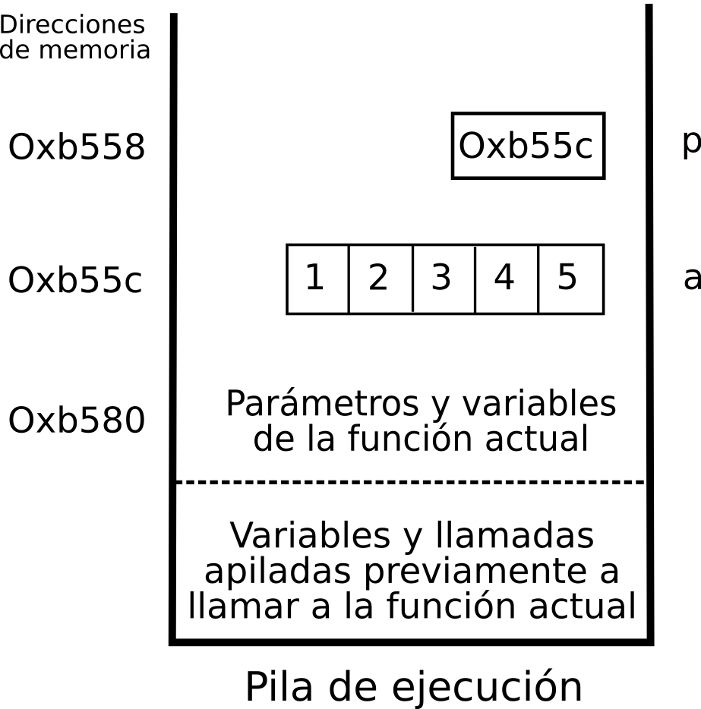
\includegraphics{imagenes/vectores-pila}
\caption{Pila de ejecución del código mostrado}
\end{figure}

Además de almacenarse de forma distinta en memoria, a un vector no se le puede
cambiar su posición en memoria, por lo que el siguiente código es inválido:

\begin{codigo-c-plano}
  int b[10];
  b = a; // ESTO NO ANDA
\end{codigo-c-plano}

En una función que recibe un arreglo por parámetro, en realidad C le pasa la
dirección de memoria del vector. Por ejemplo, si definimos la siguiente
función \lstinline!suma!:

\begin{codigo-c-plano}
  long suma(int *datos, int largo) 
  {
    long res = 0;
    for(int i = 0; i<largo; i++) {
        res += datos[i];
    }
    return res;
  }
\end{codigo-c-plano}

El puntero \lstinline!datos! tendrá la dirección de memoria del vector recibido, 
\lstinline!datos! es un puntero y no un vector.  Para invocar a la función,
podremos hacerlo de la siguiente forma:

\begin{codigo-c-plano}
    suma(a, 5); 
\end{codigo-c-plano}

Siendo \lstinline!a! el mismo vector con el que venimos trabajando. Al
poner el nombre del arreglo, C usa la dirección de memoria de \lstinline!a!
en la invocación a la función \lstinline!suma!.

En el código de \lstinline!suma! vemos que el puntero se usa exactamente
igual que como usaríamos el vector. Nuevamente, C usa la dirección del
arreglo (incluso para el operador \lstinline![i]!), por lo que el uso es
casi idéntico a utilizar un puntero.

En particular, el operador \lstinline!vector[posicion]! es exactamente lo
mismo que escribir \lstinline!*(vector+posicion)! y esto funciona ya que al
sumar un entero a una dirección de memoria el entero se multiplica por el
\lstinline!sizeof! del tipo apuntado (a esto último se lo suele llamar
\textit{aritmética de punteros}).

Para mayor claridad, el tipo de variable recibida (\lstinline!int *datos!)
se puede escribir también como \lstinline!int datos[]!, que es la forma
usual de recibir un vector en C.

\section{Vectores de vectores}

Al declarar cualquier tipo de vector, C requiere que cada posición del
vector tenga exactamente el mismo largo (en bytes), por lo que cada
posición debe ser de un tamaño fijo. 

Es por ello que, si se desea armar un vector de vectores (una matriz), se
lo deba hacer de una forma particular.  Por ejemplo, si se desea construir
una matriz de 3 filas y 4 columnas, se lo podría hacer de la siguiente
manera:

\begin{codigo-c-plano}
    int v[][4] = {{1, 2, 3, 4}, {5, 6, 7, 8}, {9, 10, 11, 12}};
\end{codigo-c-plano}

Como se ve, es posible no especificar la cantidad de filas, ya que estas se
especificarán automáticamente al inicializar, pero  es imprescindible
especificar la cantidad de columnas, ya que esto es lo que determina la
medida de cada uno de los elementos del vector \lstinline!v!.

Para acceder a la información del vector, se lo hará de la forma intuitiva:
\lstinline!v[fila][columna]!.

Hasta aquí no resulta demasiado complejo.  Las limitaciones surgen cuando
se quiere poder pasar un vector por parámetro a una función.  La forma
correcta de pasar un vector como el mostrado a una función, sería la
siguiente:

\begin{codigo-c-plano}
void imprimir_matriz(int v[][4], size_t filas);
\end{codigo-c-plano}

Es decir que la cantidad de filas puede ser variable, y se la debe recibir
por parámetro, pero la cantidad de columnas es parte del tipo de la
variable, y se la debe indicar dentro de la declaración de la función.

Esto se debe a que los elementos en memoria se guardan uno a continuación
del otro, y C necesita saber cuántos elementos tiene cada una de las
filas para poder saber cuánto se tiene que desplazar hasta encontrar el
elemento.

\section{Usar un bloque contiguo de memoria como una matriz}

Una forma de poder hacer un manejo genérico de matrices en C es basarse en que
la matriz está guardada en forma contigua en memoria y hacer la cuenta de la
posición que le corresponde a cada elemento.

Siguiendo con el ejemplo anterior, \lstinline!v! como dirección de memoria
es la dirección del elemento \lstinline!v[0][0]!. En el siguiente espacio
dentro del bloque de la memoria, que se encuentra desplazado la cantidad de
bytes que mide un entero estará \lstinline!v[0][1]!. Desplazándose cuatro
veces ese tamaño tenemos \lstinline!v[1][0]!.

Utilizando esta idea, podemos crear una nueva variable \lstinline!x!, que sea
un puntero a enteros que apunta al comienzo de \lstinline!v!. Podemos utilizar
la \emph{aritmética de punteros} vista anteriormente: haciendo
\lstinline!(x + fila*cols)! (donde \lstinline!cols! es la cantidad de
elementos por fila) obtenemos la dirección del comienzo la fila
\lstinline!fila!, esta dirección es el comienzo de un vector de enteros, por
lo que podemos hacer \lstinline!(x + fila*cols)[columna]!, para acceder al
valor de \lstinline!v[fila][columna]!.

La ventaja que obtenemos al hacer esto es que podemos escribir funciones
genéricas, que reciban el tamaño de la matriz por parámetro. Por ejemplo:

\begin{codigo-c}
void imprimir_matriz(void* aux, size_t filas, size_t cols)
{
	int *x = aux;
    for (int i=0; i < filas; i++) {
        for (int j=0; j < cols; j++) {
            printf("%d ", (x + i*cols)[j]);
        }
        printf("\n");
    }
}
\end{codigo-c}

Y la invocación a esta función sería \lstinline!imprimir_matriz(v, 3, 4)!

\section{Vectores de vectores de tamaño variable}

Teniendo en cuenta lo visto anteriormente, si se quiere crear matrices
cuyas columnas sean variables como las filas, que se las pueda pasar por
parámetro a funciones sin importar cuántas columnas tenga, será necesario
recurrir a la memoria dinámica.

Para el caso anterior, por ejemplo, se podría declarar un vector de
punteros, y cada uno de esos vectores inicializarlo como un vector de
enteros:

\begin{codigo-c-plano}
    int *w[filas];
    for (int i=0; i < filas; i++) {
        w[i] = malloc(cols*sizeof(int));
    }
\end{codigo-c-plano}

En este código, \lstinline!w! es un vector de \lstinline!filas! punteros.
Cada uno de estos punteros contiene la dirección de memoria de una porción
de memoria dinámica de tamaño \lstinline!cols*sizeof(int)!.

Al pasar este vector por parámetro a una función, se lo hará de la
siguiente manera:

\begin{codigo-c-plano}
void imprimir_matriz(int** v, size_t filas, size_t cols) {
\end{codigo-c-plano}

Utilizando este formato será posible seguir accediendo a los datos
contenidos en la matriz como \lstinline!v[fila][columna]!.

\begin{figure}[htb] 
\centering
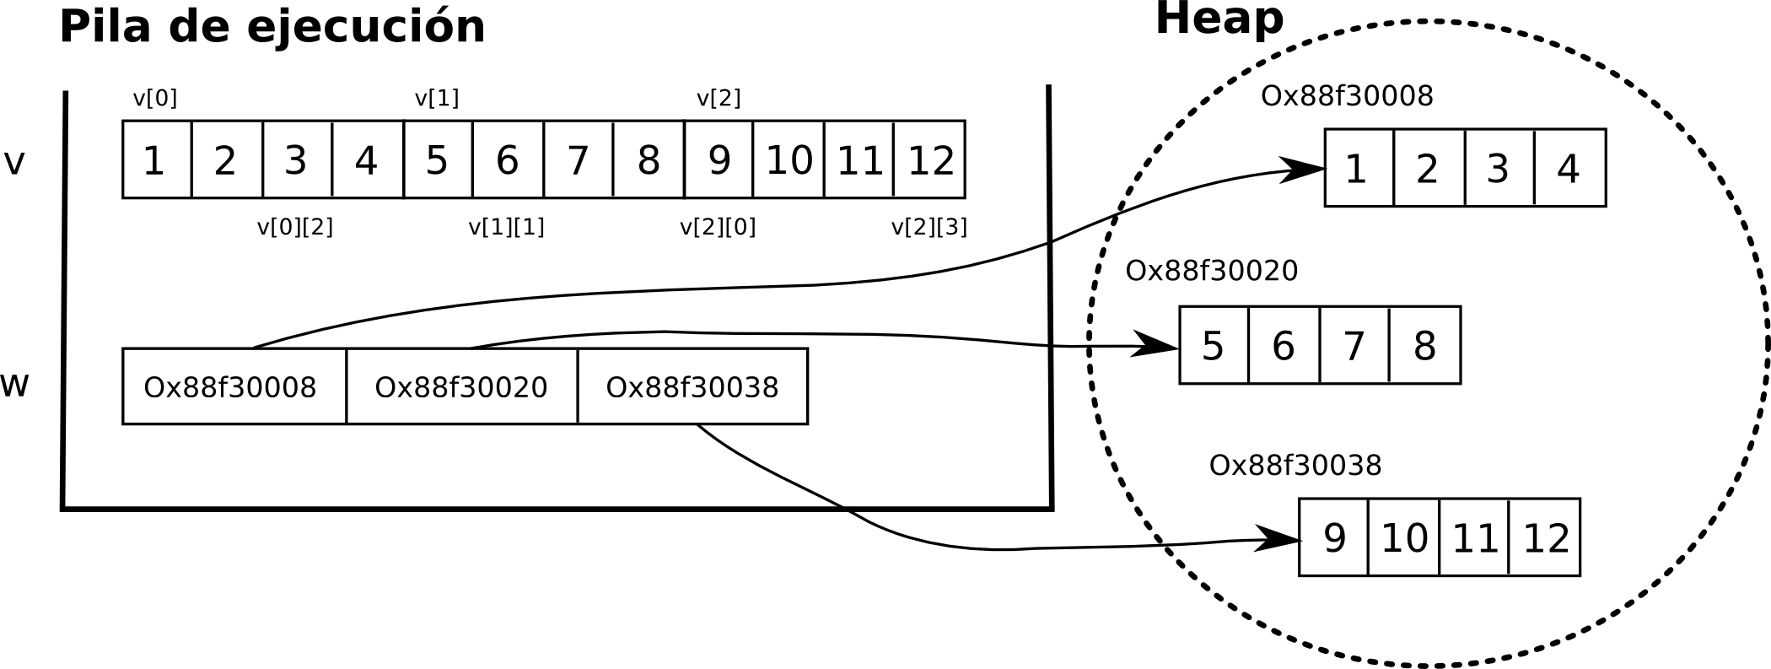
\includegraphics{imagenes/vectores-matrices}
\caption{Ubicación de los vectores mostrados en la memoria}
\end{figure}

\section{Cadenas y vectores de cadenas}

Como ya se ha mencionado, las cadenas en C son arreglos de caracteres,
terminados por un caracter \lstinline!\0!.

Si bien es posible declararlas como \lstinline!char cadena[largo]!, lo más
usual es declararlas como \lstinline!char *cadena! y luego asignar una
dirección de memoria apropiada para el dato que se quiera representar.

Cuando se declara una cadena en memoria estática, como en el siguiente
ejemplo:

\begin{codigo-c-plano}
char *cadena = "Algoritmos";
\end{codigo-c-plano}

La variable \lstinline!cadena! contiene una dirección de memoria, en la
cual comienza el arreglo de caracteres, que tiene 11 caracteres (10 letras
y un \lstinline!\0! al final). \\

Si se quiere tener un arreglo que contenga varias cadenas, se deberá operar
de manera similar a la mostrada para las matrices.

\begin{codigo-c-plano}
    char* palabras[] = {"Hola", "que", "tal"};
\end{codigo-c-plano}

Es decir que en este caso la variable \lstinline!palabras! contiene un
arreglo de tres punteros, cada uno de los cuales apunta a una porción de
memoria donde están almacenadas las palabras.




% Copyright (C) Maximiliano Curia <maxy@gnuservers.com.ar>,
%               Margarita Manterola <marga@marga.com.ar>

% Esta obra está licenciada de forma dual, bajo las licencias Creative
% Commons:
%  * Atribución-Compartir Obras Derivadas Igual 2.5 Argentina
%    http://creativecommons.org/licenses/by-sa/2.5/ar/
%  * Atribución-Compartir Obras Derivadas Igual 3.0 Unported
%    http://creativecommons.org/licenses/by-sa/3.0/deed.es_AR.
%
% A su criterio, puede utilizar una u otra licencia, o las dos.
% Para ver una copia de las licencias, puede visitar los sitios
% mencionados, o enviar una carta a Creative Commons,
% 171 Second Street, Suite 300, San Francisco, California, 94105, USA.

\renewcommand{\chaptermark}[1]{\markboth{#1}{}}
\renewcommand{\thesection}{\arabic{section}}
\chapter*{Parámetros por línea de comandos}

Se le llaman parámetros de línea de comandos a todo lo que se escriba después
del nombre del programa en la invocación de un comando. Por ejemplo, hemos
dicho que para compilar se usa una línea de la forma:

\begin{verbatim} 
gcc hola.c -o hola
\end{verbatim} 

En este caso, estamos invocando al compilador \verb!gcc! para que compile
\verb!hola.c! y genere el archivo ejecutable \verb!hola!. Esto es posible,
ya que el sistema operativo le pasa al gcc los parámetros que escribió el
usuario al invocarlo, de forma que los parámetros que recibe gcc son:

\begin{codigo-c-plano}
"gcc", "hola.c", "-o", "hola"
\end{codigo-c-plano}

En nuestro código, para recibir estos parámetros se utiliza, tradicionalmente,
la \textit{firma} de la función \lstinline!main! que recibe parámetros:
  
\begin{codigo-c-plano}
int main(int argc, char *argv[]);
\end{codigo-c-plano}

En este caso recibimos en \lstinline!main! los parámetros de la invocación
del programa.  El primer parámetro será la cantidad de parámetros que se
reciben y el segundo parámetro en un vector de punteros a caracteres.

Como se vio anteriormente, cada puntero a caracteres, es la dirección de
memoria de un bloque de caracteres.

\begin{figure}[htb]
\centering
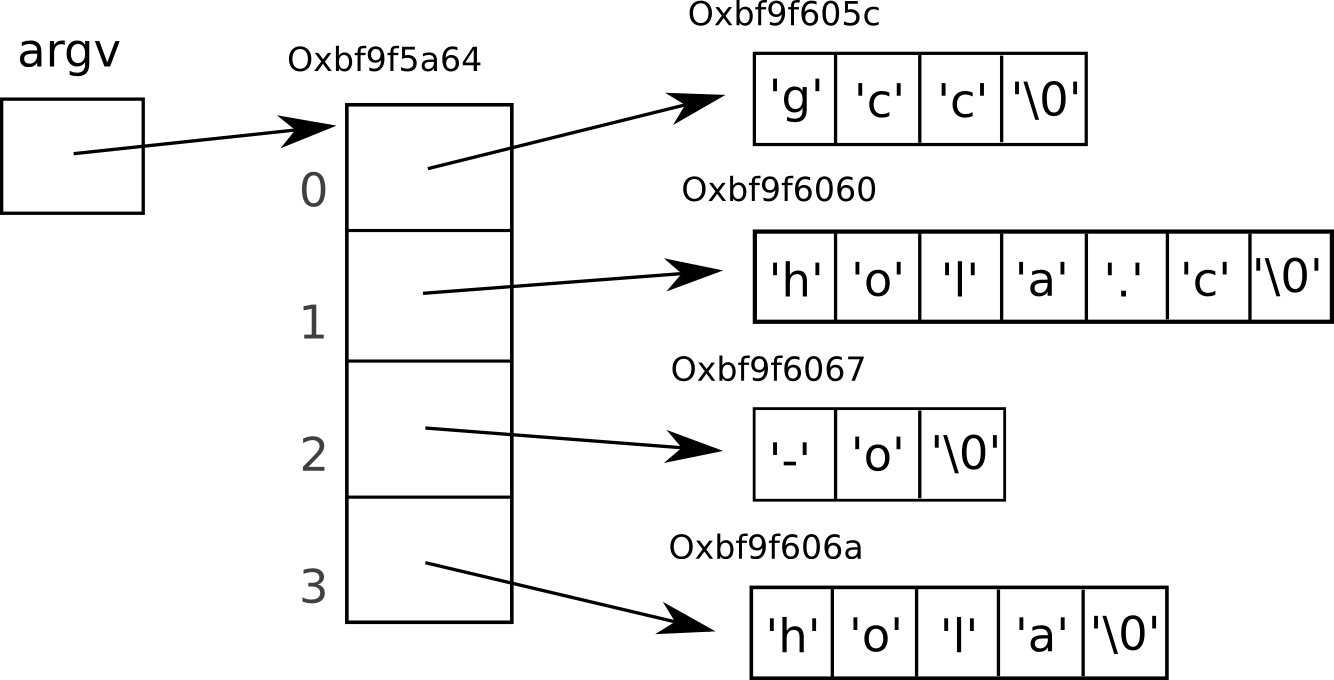
\includegraphics{imagenes/parametros}
\caption{Estructura de los parámetros recibidos por la línea de comandos
al compilar}
\end{figure}

Notar que la primera cadena apuntada por \lstinline!argv!, es el nombre del
comando que se llamó.

\section{Ejemplo de recibir parámetros por línea de comandos}

En UNIX existe un comando llamado \textbf{echo} cuya única función es imprimir todos
los parámetros que se reciben por línea de comandos. Cada parámetro se imprime
con un espacio entre parámetro y parámetro. Este sencillo programa puede
escribirse en C de la siguiente forma.

\begin{codigo-c}
#include <stdio.h>
int main(int argc, char *argv[])
{
    if (argc > 1) {
        printf("%s", argv[1]);
    }
    for (int i=2; i<argc; i++) {
        printf(" %s", argv[i]);
    }
    printf("\n");
    return 0;
}
\end{codigo-c}

En este código imprimimos todos los parámetros recibidos, omitiendo el
nombre del comando (\lstinline!argv[0]!).
Una vez compilado se lo puede invocar de la siguiente forma:
    
\begin{verbatim} 
./echo primer_parámetro  segundo_parámetro   etc
\end{verbatim} 

Y sin importar la cantidad de espacios entre un parámetro y otro el resultado
será: 

\begin{verbatim} 
primer_parámetro segundo_parámetro etc
\end{verbatim}


% Copyright (C) 2010-2013, Maximiliano Curia <maxy@gnuservers.com.ar>,
%               2010-2013, Margarita Manterola <marga@marga.com.ar>

% Esta obra está licenciada de forma dual, bajo las licencias Creative
% Commons:
%  * Atribución-Compartir Obras Derivadas Igual 2.5 Argentina
%    http://creativecommons.org/licenses/by-sa/2.5/ar/
%  * Atribución-Compartir Obras Derivadas Igual 3.0 Unported
%    http://creativecommons.org/licenses/by-sa/3.0/deed.es_AR.
%
% A su criterio, puede utilizar una u otra licencia, o las dos.
% Para ver una copia de las licencias, puede visitar los sitios
% mencionados, o enviar una carta a Creative Commons,
% 171 Second Street, Suite 300, San Francisco, California, 94105, USA.

\renewcommand{\chaptermark}[1]{\markboth{#1}{}}
\renewcommand{\thesection}{\arabic{section}}
\chapter*{Ordenamiento recursivo por mezcla, \textit{merge sort}}

El método de ordenamiento \textit{merge sort} es uno de los métodos de
ordenamiento recursivos, basados en la técnica de dividir y conquistar.  Se
lo puede utilizar para ordenar cualquier estructura secuencial (vectores,
listas, etc).

Los pasos de este método de ordenamiento son:
\begin{enumerate}
\item Cuando la longitud del vector sea 0 o 1, se considera que ya se
encuentra ordenado. De no ser así:
\item Se divide el vector en dos partes de aproximadamente la mitad del
tamaño.
\item Se ordena cada una de esas partes, utilizando este mismo método.
\item Tomando las dos partes ordenadas, se las intercala de forma ordenada,
para obtener el vector original ordenado.
\end{enumerate}

Por ejemplo, si el vector original es \verb+[6, 7, -1, 0, 5, 2, 3, 8]+, se
lo dividirá en dos partes: \verb+[6, 7, -1, 0]+ y \verb+[5, 2, 3, 8]+, que
serán ordenadas de forma recursiva.  Luego de ordenarlas, se obtendrá:
\verb+[-1, 0, 6, 7]+ y \verb+[2, 3, 5, 8]+.  Al intercalar ordenadamente
los dos vectores ordenados se obtendrá la solución buscada:
\verb+[-1, 0, 2, 3, 5, 6, 7, 8]+.

\section{Implementación básica}

Será necesario programar dos funciones.  Por un lado la función
\lstinline!merge_sort!, que será la función recursiva encargada de dividir
la lista en dos hasta llegar a la condición de corte (cuando la lista tenga
un tamaño menor que 2).

\begin{codigo-c}
void merge_sort(int vector[], int inicio, int fin)
{
    int largo = fin - inicio;
    if (largo < 2) {
        return;
    }

    int medio = inicio + (largo / 2);
    merge_sort (vector, inicio, medio);
    merge_sort (vector, medio, fin);
    merge (vector, inicio, medio, fin);
}
\end{codigo-c}

Se puede ver que esta es una función extremadamente sencilla, cuya única
tarea es dividir el vector en dos partes. Por otro lado, será necesario
programar la función \lstinline!merge!, que será la encargada de intercalar
las partes una vez que estén ordenadas.

\begin{codigo-c}
void merge (int vector[], int inicio, int medio, int fin)
{
    int pos_1 = inicio;
    int pos_2 = medio;
    int aux[fin - inicio];
    int pos_a = 0;

    // Intercala ordenadamente
    while ( (pos_1 < medio) && (pos_2 < fin) ) {
        if ( vector[pos_1] <= vector[pos_2] ) {
            aux[pos_a] = vector[pos_1];
            pos_a++; pos_1++;
        } else {
            aux[pos_a] = vector[pos_2];
            pos_a++; pos_2++;
        }
    }
    // Copia lo que haya quedado al final del primer vector
    while (pos_1 < medio) {
        aux[pos_a] = vector[pos_1];
        pos_a++; pos_1++;
    }
    // Copia lo que haya quedado al final del segundo vector
    while (pos_2 < fin) {
        aux[pos_a] = vector[pos_2];
        pos_a++; pos_2++;
    }

    // Copia los valores del vector auxiliar al original
    int a = 0;
    int i = inicio;
    while (i < fin) {
        vector[i] = aux[a];
        i++; a++;
    }
}
\end{codigo-c}

Si bien esta función tiene unas cuantas líneas de código, su tarea no es
muy compleja, simplemente inserta en un vector auxiliar los elementos del
vector que ya se encuentran ordenados, de forma que sólo se recorren los
elementos una sola vez.

\section{Análisis de complejidad}

Sea $N$ la longitud del vector. Se pueden hacer las siguientes
observaciones:

\begin{itemize}
\item En la función \lstinline!merge! se ve que el tiempo que se tarda en
intercalar dos vectores de longitud $N/2$ es proporcional a $N$, ya que
todos los elementos se copian una vez al vector auxiliar y luego se los
vuelve a copiar al vector original. Es posible, entonces, utilizar $A * N$
para representar ese tiempo.

\item Si se denomina $T(N)$ al tiempo que tarda el algoritmo en ordenar
un vector de longitud $N$, en la función \lstinline!merge_sort!
se puede ver que $T(N) = 2 * T(N/2) + A * N$, ya que la función simplemente
se llama a sí misma con dos partes de la mitad de tamaño, y luego a la
función \lstinline!merge! con el tamaño total.

\item Además, también en \lstinline!merge_sort! se puede ver que el tiempo
necesario para un vector de longitud menor a 2 es sólo el necesario en
hacer una comparación. Es decir que, $T(1) = T(0) = B$.
\end{itemize}

Estos datos forman una ecuación de recurrencia, para resolverla, se
supondrá que $N = 2^k$, quedando las ecuaciones:

\begin{eqnarray}
T(N) = T(2^k) &=&  2 * T(2^{k-1}) + A * 2^k \\
T(1) &=& B
\end{eqnarray}

Es posible resolver estas ecuaciones utilizando el \textit{método
telescópico}.

\begin{eqnarray}
T(2^k) &=& 2 * T(2^{k-1}) + A * 2^k \\
&=& 2*(2*T(2^{k-2} )+A*2^{k-1} )+A*2^k\\
&=& 2^2*T(2^{k-2} )+ 2*A(2^k)\\
&\vdots&\\
&=& 2^i* T(2^{k-i})+ i * A * 2^i\\
&\vdots&\\
&=&2^k*T(1) + k * A * 2^k\\
&=&2^k*B  + k * A * 2^k
\end{eqnarray}

Como $N = 2^k$ entonces $k=\log_2N$, y por lo que esta resolución demuestra
que $T(N) = B*N+A*N*\log_2N$.

Como $A*N*\log_2N$ es un término de mayor orden que $B*N$, el orden de este
algoritmo es $O(N*\log_2N)$.

Los valores de las constantes $A$ y $B$ son importantes a la hora de buscar
la mejor implementación de \textit{merge sort}, pero no para el cálculo del
orden del algoritmo.

Por otro lado, al analizar el espacio que consume este algoritmo, se puede
ver que para realizar el intercalado, necesita copiar el vector a un
vectora auxiliar, es decir que duplica el espacio consumido.

\section{Implementaciones más eficientes}

Si bien el orden del algoritmo \textit{merge sort} será siempre
$O(N*\log_2N)$, si se quiere una implementación realmente eficiente del
ordenamiento, será necesario hacerle algunas mejoras a la implementación
mostrada.

\subsection{Implementación con un solo pedido de memoria}

El valor $A$ está asociado al tiempo necesario para ejecutar la función
\lstinline!merge!. Una de las operaciones que se puede eliminar de esta
función es el pedido de memoria para el arreglo auxiliar,
\lstinline!int aux[fin-inicio];!, ya que esta operación consume tiempo en
pedir la memoria (y luego devolverla, al terminar la función), que podría
ahorrarse si se hiciera un único pedido de memoria para todo el algoritmo.

Para ello, será necesario crear una función adicional, que sea la que haga
el pedido de memoria auxiliar, y luego llame a la función recursiva, con
esa memoria ya reservada.

\begin{codigo-c}
void merge_sort(int vector[], int largo)
{
    int aux[largo];
    msort(vector, 0, largo, aux);
}
\end{codigo-c}

La función recursiva es ahora \lstinline!msort!, que es prácticamente igual
a la vista previamente, siemplemente incluye el pasaje de la variable
auxiliar.

\begin{codigo-c}
void msort(int vector[], int inicio, int fin, int aux[])
{
    int largo = fin - inicio;
    if (largo == 1) {
        aux[inicio] = vector[inicio];
        return;
    }

    int medio = inicio + (largo / 2);
    msort (vector, inicio, medio, aux);
    msort (vector, medio, fin, aux);
    merge (vector, inicio, medio, fin, aux);
}
\end{codigo-c}

Por otro lado, la función \lstinline!merge!, ya no deberá realizar el
pedido de memoria para alojar el vector adicional, sino que trabajará
directamente sobre la misma porción del vector auxiliar que la utilizada
para el vector de valores.

\begin{codigo-c}
void merge (int vector[], int inicio, int medio, int fin, int aux[])
{
    int pos_1 = inicio;
    int pos_2 = medio;
    int pos_a = inicio;

    // Intercala ordenadamente (...)
    // Copia lo que haya quedado al final del primer vector (...)
    // Copia lo que haya quedado al final del segundo vector (...)

    // Copia los valores del vector auxiliar al original
    int i;
    for (i = inicio; i < fin; i++) {
        vector[i] = aux[i];
    }
}
\end{codigo-c}

De esta forma se logró evitar tener que estar pidiendo memoria para el
vector auxiliar una y otra vez.  Sin embargo, esto no alcanza para decir
que se cuenta con una versión realmente eficiente de \textit{merge sort}.

\subsection{Otras mejoras}

Se puede seguir trabajando sobre el mismo algoritmo para agregarle varias
otras mejoras, como por ejemplo:

\begin{description}

\item[Implementación sin copia inútil de los datos]

Otra operación que consume tiempo inútilmente es volver a copiar los
datos del vector auxiliar al principal al terminar la función
\lstinline!merge!.

Esta copia puede evitarse si se opera alternadamente
con el vector auxiliar y con el principal, de modo que el vector auxiliar
de una llamada a \lstinline!msort! es el principal de la llamada recursiva
realizada dentro de la función, y así.

\item[Uso de otros tipos de datos]

En los ejemplos mostrados se han usado vectores de enteros para hacer más
simple el ejemplo, pero de la misma forma puede usarse cualquier otro tipo
de dato que tengamos alguna forma de compararlo. O bien hacer una
implementación que no le importe el tipo de dato con el que opera, y use
una función que recibe por parámetro para comparar elementos.

\end{description}


% Copyright (C) Maximiliano Curia <maxy@gnuservers.com.ar>,
%               Margarita Manterola <marga@marga.com.ar>

% Esta obra est� licenciada de forma dual, bajo las licencias Creative
% Commons:
%  * Atribuci�n-Compartir Obras Derivadas Igual 2.5 Argentina 
%    http://creativecommons.org/licenses/by-sa/2.5/ar/ 
%  * Atribuci�n-Compartir Obras Derivadas Igual 3.0 Unported
%    http://creativecommons.org/licenses/by-sa/3.0/deed.es_AR. 
%
% A su criterio, puede utilizar una u otra licencia, o las dos.
% Para ver una copia de las licencias, puede visitar los sitios
% mencionados, o enviar una carta a Creative Commons, 
% 171 Second Street, Suite 300, San Francisco, California, 94105, USA.

\renewcommand{\chaptermark}[1]{\markboth{#1}{}}
\renewcommand{\thesection}{\arabic{section}}
\chapter*{Ordenamiento r�pido, \textit{quick sort}}

El m�todo de ordenamiento \textit{quick sort} es el m�s famoso de los
m�todos de ordenamiento recursivos, su fama se basa en que puede ser
implementado de forma muy eficiente y en la gran mayor�a de los casos tiene
el mismo orden de complejidad que \textit{merge sort}.
Al igual que este �ltimo, est� basado en la t�cnica de dividir y conquistar.\\

Los pasos de este m�todo de ordenamiento son:
\begin{enumerate}
\item Cuando la longitud del vector sea 0 o 1, se considera que ya se
encuentra ordenado. De no ser as�:
\item Se elige un elemento del vector como \textit{pivote}.  Generalmente
ser� el primero o el �ltimo.
\item Se reordenan los elementos del vector de modo que quede dividido en
tres partes (\textbf{partici�n}): los elementos menores al pivote, el pivote y los elementos
mayores al pivote. Al terminar este paso, el pivote
queda en su lugar definitivo.
\item Se repite el mismo proceso para cada una de las partes que no
contienen al pivote (los menores y los mayores).
\end{enumerate}

Por ejemplo, si el vector original es \verb+[6, 7, -1, 0, 5, 2, 3, 8]+ y se
elige el primer elemento como pivote (\verb!6!), la partici�n del vector
ser�: \verb![-1, 0, 5, 2, 3]!, \verb!6!, \verb![7, 8]!. Se proceder� a
ordenar recursivamente \verb![-1, 0, 5, 2, 3]! y \verb![7, 8]!, de modo que
el vector final ser� \verb![-1, 0, 2, 3, 5, 6, 7, 8]!.

\section{Implementaci�n b�sica}

En este caso se implementar� una funci�n \lstinline!quick_sort!, que se
encargar� tanto de realizar la partici�n, como de llamarse recursivamente
hasta que no haya m�s elementos que ordenar.

La elecci�n del pivote depende de cada implementaci�n de \textit{quick
sort}, en este caso se elige el primer elemento del vector como pivote.

\begin{codigo-c}
void quick_sort(int vector[], int inicio, int fin)
{
    int pivote = inicio;
    int ult_menor = inicio;

    if ( (fin - inicio) < 2 ) {
        return;
    }

    int i;
    for (i = pivote + 1; i < fin; i++) {
        if ( vector[i] < vector[pivote] ) {
            ult_menor++;
            swap(vector, i, ult_menor);
        }
    }

    // Coloca el pivote al final de los menores y el �ltimo
    // menor en el primer lugar.
    swap(vector, pivote, ult_menor);
    // Ordena cada una de las mitades
    quick_sort(vector, inicio, ult_menor);
    quick_sort(vector, ult_menor+1, fin);

}
\end{codigo-c}

El bucle principal de la funci�n recorre los elementos del vector una �nica
vez, cambiando de lugar aquellos que son menores al pivote para que queden
en la primera parte y que los mayores queden en la segunda.

Una vez terminado este bucle, se coloca el pivote en el medio de ambas
partes, de modo que quede ubicado en su posici�n final.

La funci�n \lstinline!swap! utilizada en esta porci�n de c�digo, recibe un
vector y dos posiciones dentro del vector, e intercambia los valores que se
encuentran en esas dos posiciones:

\begin{codigo-c}
void swap(int vector[], int pos_1, int pos_2)
{
    int aux = vector[pos_1];
    vector[pos_1] = vector[pos_2];
    vector[pos_2] = aux;
}
\end{codigo-c}

Esta funci�n puede utilizarse siempre que se necesite intercambiar dos
elementos de un vector.

\section{An�lisis de complejidad}

A simple vista, el algoritmo de \textit{quick sort} puede parecer muy
similar al de \textit{merge sort}, ya que en ambos casos se divide a la
lista en dos, y se opera sobre partes cada vez m�s peque�as.

Sin embargo, algo importante a tener en cuenta es que en el caso del
\textit{quick sort} el orden que tenga el algoritmo depender� en una gran
parte de la elecci�n del pivote, ya que no es lo mismo elegir un valor que
se encuentre aproximadamente en el medio, de forma que las dos partes sean
aproximadamente del mismo tama�o, que elegir un valor que se encuentre en
uno de los extremos, de modo que una de las partes mida mucho m�s que la
otra.

Asumiendo que el valor elegido se encuentra aproximadamente en el medio,
se puede ver que el tiempo requerido para ejecutar el algoritmo es:

\begin{eqnarray}
T(N) &=& A * N + 2*T(N/2) \\
T(1) &=& B
\end{eqnarray}

Donde $B$ es el tiempo requerido por el caso base, y $A$ es el valor asociado
a recorrer el vector y cambiar los elementos de lugar en el bucle
principal.  Puede verse que estas ecuaciones son las mismas que para
\textit{merge sort}. \\

Sin embargo, cuando el pivote elegido no divide ambas partes al medio, el
comportamiento no es tan bueno.  En el peor caso (cuando una parte queda
con todos los elementos menos el pivote y la otra vac�a), ser�:

\begin{eqnarray}
T(N) &=& A * N + T(N-1) \\
T(1) &=& B
\end{eqnarray}

De modo que aplicando el m�todo telesc�pico, similar al utilizado
anteriormente:

\begin{eqnarray}
T(N) &=& A * N + T(N-1) \\
&=& A * N + A * (N-1) + T(N-2) \\
&=& A * (N + N - 1 + N - 2) + T(N-3) \\
&\vdots&\\
&=&A * (N + N - 1 + N - 2 + \hdots + 2) + B\\
&=&A * \sum_{i=2}^N{i} + B\\
&=&A * \frac{N^2+N}{2} - 1 + B
\end{eqnarray}

Se puede ver que en el peor caso, el orden ser� $O(N^2)$, mucho peor que el
$O(Nlog_2N)$ visto anteriormente.  Sin embargo, se pueden tomar recaudos
especiales para que este peor caso sea extremadamente improbable, y que en
la pr�ctica se pueda considerar que el algoritmo se comporta como
$O(Nlog_2N)$.

\section{Implementaciones m�s eficientes}

\subsection{Elecci�n del pivote}

Si se elige el primer elemento (o el �ltimo), el algoritmo resulta muy
inconveniente para el caso de una lista que ya se encuentra ordenada, y
este es un caso que en ciertas situaciones es esperable que suceda.

Es por eso que una optimizaci�n sencilla es intercambiar el elemento del
medio con el que se vaya a utilizar de pivote antes de comenzar el bucle
principal.

\begin{codigo-c}
    int medio = (fin + inicio) / 2;
    swap(vector, pivote, medio);
\end{codigo-c}

Otras t�cnicas de elecci�n del pivote incluyen:
\begin{itemize}
\item Elegir un elemento aleatoriamente, esto hace que en promedio sea
mucho m�s probable tener un buen caso que uno malo, pero no elimina la
posibilidad del peor caso.
\item Recorrer la lista y buscar el elemento que ocupar� la posici�n
central de la lista.  Eso asegura que el orden sea siempre $O(Nlog_2N)$, pero
decrementa mucho la eficiencia del caso base.
\item Elegir tres elementos de la lista (por ejemplo, el primero, el del
medio y el �ltimo), y quedarse con el del medio de los tres como pivote.
\end{itemize}

\subsection{Reducci�n de la cantidad de intercambios}

En la implementaci�n vista, puede suceder que se hagan numerosos
intercambios innecesarios, cuando un elemento ya es menor que el pivote, y
simplemente har�a falta avanzar la variable que indica la posici�n del
�ltimo menor.

Una implementaci�n alternativa de {\it quick sort} se basa en esta idea para
tratar de minimizar la cantidad de intercambios.  Se cuenta con dos
variables, que se utilizan para saltear los elementos que no hace falta
cambiar de lugar, y s�lo cambiar aquellos que es necesario.

\begin{codigo-c}
void quick_sort(int vector[], int inicio, int fin)
{
    if ( (fin - inicio) < 2 ) {
        return;
    }
    int izq = inicio + 1;
    int der = fin - 1;
    int pivote = inicio;

    // Cambia el del medio con el primero. 
    // (optimizaci�n para vectores ordenados).
    int medio = (izq + der) / 2;
    swap(vector, pivote, medio);

    while (izq <= der) {
        while ( (izq <= der) && (vector[der] >= vector[pivote]) )
            der--;
        while ( (izq <= der) && (vector[izq] < vector[pivote]) )
            izq++;
        if ( izq < der )
            swap(vector, izq, der);
    }

    // Coloca el pivote al final de los menores y el �ltimo
    // menor en el primer lugar.
    swap(vector, pivote, der);
    // Ordena cada una de las mitades
    quick_sort(vector, inicio, der);
    quick_sort(vector, der+1, fin);
}
\end{codigo-c}

Como se puede ver, se ha reemplazado el bucle principal, por otro que
recorre el vector desde ambas puntas hacia el medio, buscando los elementos
que necesitan ser intercambiados.

\subsection{Utilizaci�n de otros algoritmos}

En particular para los casos de las partes m�s peque�as, al tener menos
elementos, sin importar cu�l se elija como pivote, es m�s probable que se
asemejen al peor caso.

Es por ello que una t�cnica de optimizaci�n puede incluir utilizar un
algoritmo alternativo, como por ejemplo el de ordenamiento por inserci�n,
para secuencias de pocos elementos. \\

Por otro lado, puede tambi�n implementarse un contador que verifique la
profundidad de la recursi�n y cuando esta exceda el nivel esperado por el
algoritmo, pasar a utilizar otro algoritmo de ordenamiento, como {\it merge
sort} o {\it heap sort}.

\section{Quick sort en la biblioteca est�ndar de C}

Entre las funciones que provee la biblioteca est�ndar de C, se incluye una
implementaci�n de quick sort. Dado que la biblioteca est�ndar est� altamente
probada y seguramente contenga optimizaciones avanzadas, es en general una
buena idea usar las funciones que provistas antes que usar las propias.

En el caso del \textit{quick sort}, la funci�n se llama \lstinline!qsort! y se
encuentra definida en el encabezado \lstinline!<stdlib.h>!, su prototipo es:

\begin{codigo-c}
void qsort(void *base, size_t nmemb, size_t size,
           int(*compar)(const void *, const void *));
\end{codigo-c}

Que puede ser intimidante por la cantidad y complejidad de par�metros que
recibe, en gran parte debido a la generalidad del c�digo. \lstinline!base! se
refiere al vector a ordenar, \lstinline!nmemb! es la cantidad de elementos
del vector, \lstinline!size! es el tama�o en bytes de un elemento,
\lstinline!compar! es la funci�n que se debe usar para comparar.

Este tipo de funciones se ver�n con m�s detalle m�s adelante.


% Copyright (C) 2010-2013, Maximiliano Curia <maxy@gnuservers.com.ar>,
%               2010-2013, Margarita Manterola <marga@marga.com.ar>

% Esta obra está licenciada de forma dual, bajo las licencias Creative
% Commons:
%  * Atribución-Compartir Obras Derivadas Igual 2.5 Argentina
%    http://creativecommons.org/licenses/by-sa/2.5/ar/
%  * Atribución-Compartir Obras Derivadas Igual 3.0 Unported
%    http://creativecommons.org/licenses/by-sa/3.0/deed.es_AR.
%
% A su criterio, puede utilizar una u otra licencia, o las dos.
% Para ver una copia de las licencias, puede visitar los sitios
% mencionados, o enviar una carta a Creative Commons,
% 171 Second Street, Suite 300, San Francisco, California, 94105, USA.

\renewcommand{\chaptermark}[1]{\markboth{#1}{}}
\renewcommand{\thesection}{\arabic{section}}
\chapter*{Compilación de varios archivos en C}

En todo programa es importante modularizar el código de forma que se facilite
la reutilización y se minimice la repetición de código.
En particular, cuando se trata de tipos abstractos de datos, es importante
tener un módulo correspondiente a cada tipo abstracto.

Por otro lado, para que un tipo abstracto de datos sea realmente
\textit{abstracto} es recomendable que la implementación de las operaciones
correspondientes al tipo estén separadas de los prototipos de estas
operaciones, de modo que quien las utiliza se concentre únicamente en cuáles
son las operaciones y no en cómo se llevan a cabo.

\section{Encabezado, implementación y código objeto}

En C, esto se logra mediante la separación de cada módulo en un archivo
\verb!.h!, que contiene las declaraciones de estructuras, constantes y
prototipos de las funciones, que es llamado el \textit{encabezado} del módulo,
y un archivo \verb!.c! que contiene las implementaciones correspondientes.

Cada uno de los archivos \verb!.c! se utiliza para generar un archivo
\verb!.o! que contiene el \textit{código objeto}, es decir el código de
máquina, correspondiente a cada módulo.

Cuando se compila un programa completo, todos los \verb!.o! que se hayan
generado a partir de los módulos programados deben combinarse en un sólo
ejecutable.

\subsection{Inclusión de otros encabezados}

Cuando un módulo requiere de funciones definidas en otros módulos, debe
incluir los encabezados (los archivos \verb!.h!) en los que esas funciones
están definidas.  Esta inclusión se realiza normalmente dentro del encabezado
correspondiente al módulo en cuestión.

Es posible que al momento de construir un programa de tamaño considerable
suceda que hay varios módulos que dependen de otro. De modo que podría suceder
que este otro se incluya varias veces, lo cual es problemático y debe ser
evitado.

Para solucionar este problema, se utilizan las construcciones condicionales
del preprocesador, haciendo que el código definido dentro de un encabezado se
incluya en el programa un única vez. Por ejemplo:

\begin{codigo-c-plano}
#ifndef __ENUM_H
    #define __ENUM_H
    typedef enum {OK, ERROR} estado;
    typedef enum {HUMANO, COMPUTADORA} jugador_t;
#endif
\end{codigo-c-plano}

En este caso, el preprocesador verifica si está definida la variable
\lstinline!__ENUM_H!. De no estar definida, la define y luego define los tipos
enumerados correspondientes a este encabezado.

En cambio, si la variable ya estaba definida, significa que este encabezado ya
fue procesado, con lo cual no se hace nada.


\section{Compilación con \texttt{make}}

Cuando los módulos que componen un programa son muchos, los pasos necesarios
para compilarlo pueden ser muchos y tener que regenerarlos manualmente cada
vez que se los modificque sería una tarea demasiado tediosa.  Es por ello que
existe una herramienta llamada \verb!make!, encargada de realizar todos los
pasos de compilación y necesarios y de hacerlos sólo cuando haga falta.

Esta herramienta utiliza, a modo de configuración, los archivos
\verb!Makefile! en donde se indican los pasos a realizar para la compilación
tanto de los módulos como del programa principal.

En estos archivos, básicamente, se pueden definir variables y reglas para
compilar los distintos módulos.

\subsection{Un \texttt{Makefile} sencillo}

A continuación un ejemplo de cómo puede verse un posible archivo
\verb!Makefile!.

\begin{lstlisting}[language=make, numbers=none]
CFLAGS = -g -Wall -std=c99
EXEC = miprog
OBJ = lista.o pila.o
CC = gcc

all: $(EXEC)

lista.o: lista.c lista.h
	$(CC) $(CFLAGS) -c lista.c

pila.o: pila.c pila.h
	$(CC) $(CFLAGS) -c pila.c

$(EXEC): $(OBJ) miprog.c
	$(CC) $(CFLAGS) $(OBJ) miprog.c -o $(EXEC)
\end{lstlisting}

\subsection{Variables}

En la primera parte se declaran 4 variables, \lstinline!CFLAGS! son los
\textit{flags} (parámetros) de compilación utilizados, en este caso se trata
del parámetro que incluye la información para depuración \lstinline!-g! y el
parámetro para que advierta sobre todos los posibles problemas que el
compilador encuentre, \lstinline!-Wall!.

Luego se declara el nombre que tendrá el programa ejecutable.  En este caso no
tiene extensión, puesto que es un programa para sistemas UNIX (Linux, BSD,
Solaris, etc). Si se estuviera compilando para un sistema Windows, la variable
\lstinline!EXEC! sería \lstinline!miprog.exe!.

Luego se listan cuáles serán los módulos que deberán transformarse en código
objeto, y finalmente se coloca el nombre del compilador.  Separar la
información de esta manera permite que si es necesario hacer un cambio en la
forma de compilar un programa, el trabajo para realizarlo sea mínimo.

Es importante notar que en el \verb!Makefile!, las variables se definen
simplemente con \lstinline!VARIABLE=VALOR!, pero luego para utilizarlas, se lo
hace de la forma \lstinline!$(VARIABLE)!.

\subsection{Reglas de compilación}

Luego de las variables, se definen cada uno de los archivos a generar, los
archivos de los cuales estos dependen, y las acciones a llevar a cabo para
compilar los archivos correspondientes.

Cuando se ejecuta el comando \verb!make! sin ningún parámetro, se ejecuta
automáticamente la primera de todas las reglas, es por eso que esta regla
normalmente se llama \lstinline!all! y simplemente indica cuál es el archivo a
generar.

Luego de esta regla especial, se encuentran las reglas de compilación de cada
uno de los módulos del programa.  Las reglas tienen un formato específico que
se debe cumplir para que funcione el \verb!Makefile!.

\begin{lstlisting}[language=make, numbers=none]
archivo: dependencias
	acciones
\end{lstlisting}

Esto significa que \lstinline!archivo! debe generarse cada vez que
cambie una de las \lstinline!dependencias!, ejecutando las
\lstinline!acciones!.

Es importante notar que para que el \verb!make! funcione correctamente, las
acciones a realizar deben tener un tabulador de separación desde el comienzo
de línea.  Puede haber más de una acción, de a una por línea, siempre que se
mantenga un tabulador de separación. \\

En particular, la regla que se encarga de generar el programa principal es
diferente a las otras, ya que incluye una mayor cantidad de dependencias y de
variables.

\begin{lstlisting}[language=make, numbers=none]
$(EXEC): $(OBJ) miprog.c
	$(CC) $(CFLAGS) $(OBJ) miprog.c -o $(EXEC)
\end{lstlisting}

Esta regla indica que el archivo indicado mediante la variable
\lstinline!$(EXEC)! definida previamente debe generarse cuando cambie cualquiera
de los archivos objeto, ya que si estos cambian, también debe cambiar el
ejecutable final, o bien si cambia el código principal del programa. \\

Es importante notar que mediante estas reglas, \verb!make! no sólo es capaz de
compilar los archivos de forma correcta, sino que también es capaz de
realizarlo sólo cuando sea necesario.  Para ello, verifica que la fecha de
modificación de los archivos listados como dependencias sea anterior al
archivo a generar.  De no ser así, vuelve a generarlo, ya que algo ha
cambiado.

\subsection{Reglas genéricas}

Cuando la gran mayoría de los archivos del programa se compilan de una misma
forma, es posible simplificar el archivo \verb!Makefile!, mediante el uso de reglas
genéricas.

Por ejemplo, para el caso del \verb!Makefile! visto anteriormente, las dos
líneas que generan los archivos \verb!.o! podrían simplificarse en una sola de
la siguiente forma:

\begin{lstlisting}[language=make, numbers=none]
%.o: %.c %.h
	$(CC) $(CFLAGS) -c $<
\end{lstlisting}

Esta regla significa que para generar un archivo \verb!.o! es necesario contar
con un archivo del mismo nombre \verb!.c! y otro del mismo nombre \verb!.h!.
En la regla de compilación se utiliza la variable especial \lstinline!$<!, que
toma el valor de la primera de las dependencias listadas (el archivo
\verb!.c!.).  Existe también \lstinline!$@!, que toma el nombre del archivo
que está siendo generado en esa regla.

\subsection{Acciones comunes}

Además de compilar, es común querer eliminar los archivos generados, de modo
que queden únicamente los archivos fuente del programa.  Esta acción
normalmente se realiza mediante una regla especial llamada \lstinline!clean!.

Si bien puede llevar cualquier nombre, lo más usual es ponerle este nombre ya
que tanta gente la llama así que cualquier programador que se encuentre con un
\verb!Makefile! esperará encontrar una regla con este nombre que realice esta
acción.

\begin{lstlisting}[language=make, numbers=none]
clean:
	rm $(OBJ) $(EXEC)
\end{lstlisting}

Para utilizar esta regla (o cualquier otra que no sea la predeterminada), debe
invocarse el comando \verb!make! con el nombre de la regla como parámetro. Es
decir, \verb!make clean!.

Al igual que con \lstinline!clean!, existen otras acciones comunes que se
suelen incluir en la mayoría de los programas.  Las más conocidas:

\begin{description}
\item[build] Para compilar el código (equivalente a la regla
\lstinline!all! del ejemplo mostrado).
\item[install] Para instalar el código compilado en el sistema.
\item[uninstall] Para desinstalar el programa que haya sido
instalado.
\end{description}

\subsection{Variables comunes}

Así como existen reglas comunes, que la mayoría de los programadores están
acostumbrados a encontrar en los archivos \verb!Makefile!, también existen
variables que suelen estar presentes.

\begin{description}
\item[CFLAGS] Que estaba en el ejemplo mostrado, son los
parámetros pasados al compilador.
\item[LDFLAGS] Son los parámetros pasados al enlazador.
\item[PREFIX] Utilizado cuando hay una regla de instalación, es el
directorio a partir del cual se instalarán los archivos.
\end{description}

\subsection{Reglas, archivos y PHONY}

Cada regla de makefile tiene como finalidad crear un archivo, sin embargo hay
reglas como la regla \verb!clean! que mostramos más arriba que no genera
ningún archivo, tampoco depende de ningún archivo (de hecho borra archivos,
pero esto es parte de la acción y a make no le importa que hace la acción).

Es más, si creamos un archivo llamado \verb!clean! make creerá que la regla
está satisfecha. Para evitar que \verb!make! revise archivos que no vamos a
generar es de bastante recomendable declarar las reglas que no generan
archivos como \verb!.PHONY!, por ejemplo:

\begin{lstlisting}[language=make, numbers=none]
.PHONY: install clean
\end{lstlisting}


%% Copyright (C) 2010-2013, Maximiliano Curia <maxy@gnuservers.com.ar>,
%               2010-2013, Margarita Manterola <marga@marga.com.ar>

% Esta obra está licenciada de forma dual, bajo las licencias Creative
% Commons:
%  * Atribución-Compartir Obras Derivadas Igual 2.5 Argentina
%    http://creativecommons.org/licenses/by-sa/2.5/ar/
%  * Atribución-Compartir Obras Derivadas Igual 3.0 Unported
%    http://creativecommons.org/licenses/by-sa/3.0/deed.es_AR.
%
% A su criterio, puede utilizar una u otra licencia, o las dos.
% Para ver una copia de las licencias, puede visitar los sitios
% mencionados, o enviar una carta a Creative Commons,
% 171 Second Street, Suite 300, San Francisco, California, 94105, USA.

\renewcommand{\chaptermark}[1]{\markboth{#1}{}}
\renewcommand{\thesection}{\arabic{section}}
\chapter*{Archivos en C}

En este apunte se verá una referencia de las funciones y conceptos de archivos
usado en C, resaltando algunas peculiaridades que no se ven en otros
lenguajes. Pero de ninguna manera pretende ser un apunte completo sobre el uso
de archivos en general y se asume cierta experiencia al respecto.

Una de las peculiaridades de C es que, todos los programas al ejecutarse ya
tienen tres archivos abiertos, estos son: la entrada estándar
(\textit{stdin}), salida estándar (\textit{stdout}) y salida de error
(\textit{stderr}). Los primeros dos son los que usan las funciones de entrada
y salida del usuario, como \lstinline!scanf!  y \lstinline!printf!,
respectivamente. El tercero es un archivo de salida destinado al envío de
errores de ejecución y por omisión saldrán en la misma salida que los de
salida externa.

Siendo que lo que tiene que ver con archivos es normalmente entrada o salida
del programa, las funciones listadas en este apunte están declaradas en el
encabezado \lstinline!<stdio.h>!.

\section{Entrada y salida de una terminal}

La entrada y salida de una terminal en C se comporta de una forma similar a la
lectura y escritura de archivos, por lo que se listan a continuación algunas
de las funciones de entrada y de salida.

Tanto la entrada como la salida estándar suelen tener un \textit{buffer}, es
decir una memoria intermedia, en este caso por líneas, por lo que al intentar
leer de entrada estándar mediante \lstinline!scanf!, el programa se quedará
esperando hasta que se termine una línea en la entrada, aún si sólo se quiere
leer un caracter. El resto de línea no procesada será la entrada de las
siguientes llamadas a las funciones de entrada.

Algo similar sucede con la salida por consola, cuando se utiliza
\lstinline!printf!, la salida suele tener también un \textit{buffer} orientado
a líneas, por lo que hasta que no se termine una línea, la salida no se emite
en la terminal.

\subsection{Manejo de caracteres de a uno}

Sin embargo, no es la única opción.  Existen otras funciones como:

\begin{codigo-c-plano}
int getchar(void);
\end{codigo-c-plano}

Esta función permite leer un único caracter desde la entrada estándar,
devuelve el valor del caracter leído o, en caso de haberse terminado la
entrada, el valor especial \lstinline!EOF!.

De la misma forma, para emitir un único caracter por la terminal:

\begin{codigo-c-plano}
int putchar(int c);
\end{codigo-c-plano}

Esta función permite escribir un caracter en la terminal, devuelve el valor
del caracter escrito o bien \lstinline!EOF! en caso de error.

% %%%% scanf y printf ya estaban, pero se podría completar mejor.

%\subsection{Entrada y salida con formato}
%
%Como ya se ha visto previamente, para una lectura con formato se utiliza
%\lstinline!scanf!\footnote{Para más información: \texttt{man 3 scanf}.},
%cuyo prototipo es:
%
%\begin{codigo-c-plano}
%int scanf(const char *formato, ...);
%\end{codigo-c-plano}
%
%El primer parámetro es una cadena de formato, que define, entre otras cosas,
%los tipos de las variables a leer. El \lstinline!...!, es una forma de
%declarar una función que recibe una cantidad arbitraria de parámetros. En este
%caso, en esa ubicación van las direcciones de memoria en las que se deben
%escribir los datos leidos. El valor devuelto es la cantidad de valores leidos,
%que puede ser menor a la cantidad pedida, o bien \lstinline!EOF! en caso de
%error.
%
%Para emitir valores por la terminal usamos \lstinline!printf!\footnote{Para
%más información \texttt{man 3 scanf}.}, cuyo prototipo es:
%
%\begin{codigo-c-plano}
%int printf(const char *formato, ...);
%\end{codigo-c-plano}
%
%El primer parámetro es una cadena de formato, que define, entre otras cosas,
%los tipos de las variables a emitir. Los siguientes parámetros serán los
%valores a imprimir.

% %%% Cadena de formato

\section{Abrir archivos}

Para abrir un archivo en C se utiliza la función
\lstinline!fopen!\footnote{Para más información: \texttt{man 3 fopen}.}, cuyo
prototipo es:

\begin{codigo-c-plano}
FILE *fopen(const char *ruta, const char *modo);
\end{codigo-c-plano}

El primer parámetro es el nombre del archivo, y el segundo el modo de
apertura, que puede ser:

\begin{tabular}{lp{10cm}}
\verb!r!  & Sólo lectura, se posiciona al principio del archivo. \\
\verb!r+! & Lectura y escritura, se posiciona al principio del archivo. \\
\verb!w!  & Borra el contenido del archivo o crea uno nuevo, sólo escritura, se
posiciona al principio del archivo. \\
\verb!w+! & Borra el contenido del archivo o crea uno nuevo, lectura y
escritura, se posiciona al principio del archivo. \\
\verb!a!  & Abre para añadir (escribir al final del archivo). El archivo se
crea si no existe. Se posiciona al final del archivo. \\
\verb!a+! & Abre para leer y añadir (escribir al final del archivo). El
archivo se crea si no existe. Se posiciona al final del archivo.\\
\end{tabular}

Además, el archivo puede abrirse en modo \emph{archivo de texto} (por omisión)
o en modo \emph{archivo binario} (agregándole una \verb!b! al modo). Los
archivos de texto tienen un tratamiento especial para el caracter fin de
línea, mientras que con los archivos binarios se accede a los datos en crudo.

El valor devuelto por \lstinline!fopen! es un puntero de tipo
\lstinline!FILE! que representa a los archivos en la biblioteca estándar. En
caso de error, el valor devuelto es \lstinline!NULL!.

\section{Cerrar archivos}

Cerrar un archivo es más sencillo:

\begin{codigo-c-plano}
int fclose(FILE *archivo);
\end{codigo-c-plano}

Devuelve \lstinline!0! si tuvo exito, o \lstinline!EOF! en caso de error.

\section{Leer o escribir de un archivo}

De la misma manera que \lstinline!getchar!  para leer un caracter de la
entrada estándar, existe \lstinline!fgetc!  \footnote{Para más información:
\texttt{man 3 fgetc}.} para leer un único caracter de un archivo.

\begin{codigo-c-plano}
int fgetc(FILE *archivo);
\end{codigo-c-plano}

De hecho, la siguiente función es prácticamente equivalente a la función
\lstinline!getchar()!.

\begin{codigo-c-plano}
int mi_getchar(void)
{
	return fgetc(stdin);
}
\end{codigo-c-plano}

De la misma forma, existen \lstinline!fputc!, para escribir un caracter a un
archivo, \lstinline!fscanf!, para leer con formato de un archivo,
\lstinline!fprintf!  un archivo.\footnote{Para más información: \texttt{man
3 fputc}, \texttt{man 3 fscanf}, \texttt{man 3 fprintf}.}, para escribir con
formato a Sus prototipos son:

\begin{codigo-c-plano}
int fputc(int c, FILE *archivo);
int fscanf(FILE *archivo, const char *formato, ...);
int fprintf(FILE *archivo, const char *formato, ...);
\end{codigo-c-plano}

Además de estas funciones existen:

\begin{codigo-c-plano}
char *fgets(char *buffer, int tamanio, FILE *archivo);
int fputs(const char *buffer, FILE *archivo);
\end{codigo-c-plano}

La función \lstinline!fgets! lee el archivo hasta encontrar un fin de línea,
un fin de archivo o haber llegado a leer \lstinline!tamanio! bytes. Cuando lee
un fin de línea lo deja en el \lstinline!buffer!. Devuelve la dirección del
\lstinline!buffer! o bien \lstinline!EOF! si se trata de leer estando al final
del archivo.

La función \lstinline!fputs! escribe la cadena apuntada por \lstinline!buffer!
en \lstinline!archivo!. Devuelve la cantidad de bytes escritos o bien
\lstinline!EOF! en caso de error.

Las funciones \lstinline!fgets! y \lstinline!fputs! constituyen la forma
estándar de leer o escribir líneas en un archivo, si bien puede suceder que lo
que se lea no sea una línea completa (cuando la línea ocupa más espacio que
\lstinline!tamanio!.

Si bien tienen un paralelo que trabaja sobre la entrada y salida estándar,
esas funciones no se utilizan ya que pueden dar lugar a varios problemas de
seguridad.

\section{Otras funciones de archivos}

Otras funciones que vale la pena mencionar son:

\begin{codigo-c-plano}
int fflush(FILE *archivo);
int feof(FILE *archivo);
\end{codigo-c-plano}

La función \lstinline!fflush! fuerza la escritura de los buffers que estén
pendientes en el archivo. Devuelve 0 si se ejecutó correctamente, o
\lstinline!EOF! en caso de error. Puede utilizarse para evitar el
comportamiento del buffer por líneas de las salida estándar.

La función \lstinline!feof! devuelve algo distinto de cero si se encuentra al
final del archivo o \lstinline!0! en caso contrario.

\section{Archivos binarios}

Los archivos de texto son sencillos de procesar y faciles de leer aún fuera
del programa que los usa, el éxito en los últimos años de los formatos XML,
HTML, SVG, etc, demuestra su gran flexibilidad. Por otro lado, los archivos
binarios permiten almacenar la información de forma que sea muy eficiente
acceder a ella.

El formato a utilizar en una aplicación se debe decidir según el uso que se le
vaya a dar a los archivos, si se quiere que sean legibles por seres humanos,
si se quiere poder compartir la información entre aplicaciones, o si
simplemente se quiere poder leer y guardar la información de la forma más
eficiente.

%Es parte del trabajo de un programador decidir el formato de datos a utilizar,
%por suerte para nosotros esto se ve con mucho más detalle en otra materia. :)

Las funciones vistas hasta ahora son las más utilizadas al trabajar sobre
archivos de texto, estas pueden servir para archivos binarios, pero además se
necesitarán las siguientes:

\begin{codigo-c-plano}
size_t fread(void *buffer, size_t tamanio, size_t cantidad, FILE *archivo);
size_t fwrite(const void *buffer, size_t tamanio, size_t cantidad,
              FILE *archivo);
\end{codigo-c-plano}

La función \lstinline!fread! lee \lstinline!cantidad! bloques de bytes de
\lstinline!tamanio! bytes cada uno, de un archivo, almacenandolos en
\lstinline!buffer!. Devuelve la cantidad de elementos leídos del archivo, en
el caso de estar en el final del archivo devolverá 0.

De la misma forma \lstinline!fwrite! escribe \lstinline!cantidad! bloques de
bytes de \lstinline!tamanio! bytes cada uno en archivo y devuelve la cantidad
de elementos escritos.

\begin{codigo-c-plano}
int fseek(FILE *archivo, long desplazamiento, int origen);
\end{codigo-c-plano}

Se mueve dentro el archivo, \lstinline!desplazamiento! es un valor relativo a
\lstinline!origen!, puede referirse al principio del archivo
(\lstinline!SEEK_SET!), a la posición actual (\lstinline!SEEK_CUR!) o al final
del archivo (\lstinline!SEEK_END!). El valor devuelto será 0 en caso de exito
o \lstinline!-1! en caso de error.

\begin{codigo-c-plano}
long ftell(FILE *archivo);
\end{codigo-c-plano}

Devuelve la posición actual del archivo, o \lstinline!-1! en caso de error.

\section{Ejemplo: Copiar un archivo}

\begin{codigo}{copiar.c}{Copia un archivo}
\begin{codigo-c-plano}
#include <stdio.h>
#include <stdlib.h>

int main(void)
{
	FILE *origen, *destino;
	int  valor;

	origen = fopen("copiar.c","r");
	if ( origen == NULL ) {
		fprintf(stderr, "Error al abrir el archivo origen");
		exit(1);
	}

	destino = fopen("copiar2.c","w");
	if ( destino == NULL ) {
		fprintf(stderr, "Error al abrir el archivo destino");
		exit(1);
	}

	do {
		valor = fgetc(origen);
		if ( valor != EOF ) {
			fputc(valor,destino);
		}
	} while (valor != EOF);
	fclose(origen);
	fclose(destino);

	return 0;
}
\end{codigo-c-plano}
\end{codigo}

En este ejemplo vemos el uso de varias de las funciones mencionadas
anteriormente. El código copia un archivo de un forma muy ineficiente,
leyendolo de 1 caracter. Se muestra también el uso de \lstinline!stderr!.

Podemos mejorarlo un poco leyendo por lineas en vez de caracter a caracter.

\begin{codigo-c-plano}
enum {MAXLINE = 1024};
...
	char buffer[MAXLINE], *aux;
	do {
		aux = fgets(buffer, MAXLINE, origen);
		if ( aux != NULL ) {
			fputs(buffer, destino);
		}
	} while (aux != NULL);
\end{codigo-c-plano}

Se puede mejorar la eficiencia de este código utilizando \lstinline!fread! y
\lstinline!fwrite!.

% Tomar los nombres de archivo por parámetro
% Y usar stdin y stdout si no se especifican.
% TODO: Falta, freopen


%\include{apendice}
%\include{referenc}
%
\chapter*{Licencia y Copyright}
\addcontentsline{toc}{chapter}{Licencia y Copyright}

{\noindent
Copyright \copyright\ 2010-2013, Maximiliano Curia <maxy@gnuservers.com.ar> \\
Copyright \copyright\ 2010-2013, Margarita Manterola <marga@marga.com.ar> \\
}

Esta obra está licenciada de forma dual, bajo las licencias Creative Commons: 

\begin{itemize}
\item Atribución-Compartir Obras Derivadas Igual 2.5 Argentina \\ http://creativecommons.org/licenses/by-sa/2.5/ar/
\item Atribución-Compartir Obras Derivadas Igual 3.0 Unported \\ http://creativecommons.org/licenses/by-sa/3.0/deed.es\_AR.
\end{itemize}

A su criterio, puede utilizar una u otra licencia, o las dos. Para ver una copia de las licencias, puede visitar los sitios mencionados, o enviar una carta a Creative Commons, 171 Second Street, Suite 300, San Francisco, California, 94105, USA.

%\typeout{Bibliography}

%\addcontentsline{toc}{chapter}{Referencias}

%\bibliography{referenc}
%\bibliographystyle{alpha}

\end{document}
